%-  LaTeX source file

%-  section4.tex ~~
%
%   This is the fourth section of the paper.
%
%                                                   ~~ last updated 29 Aug 2019

%%%%%%%%%%%%%%%%%%%%%%%%%%%%%%%%%%%%%%%%%%%%%%%%%%%%%%%%%%%%%%%%%%%%%%%%%%%%%%%

In 2013, the PanDA team began working to incorporate the Titan supercomputer at
Oak Ridge National Laboratory as a grid site for the Worldwide LHC Compute
Grid, on behalf of the ATLAS Collaboration. The team has operated under several
different project identifiers, including CSC108, HEP110, and HEP113. The HEP110
and HEP113 projects represent traditional ASCR Leadership Computing Challenge
(ALCC) allocations, but the CSC108 project operates exclusively in what the
team has colloquially referred to as ``backfill mode'', which is outlined in
Section~\ref{sec:deploying}. The goal of CSC108 has been to consume idle
resources on Titan which would otherwise have gone to waste, while making a
good-faith effort not to disturb the rest of Titan's ecosystem. The focus of
this section is to assess the degree to which CSC108 has accomplished this goal
and especially to analyze the impact of the project on Titan.

% SOMEWHERE, there needs to be discussion of the constraints that face CSC108,
% and also there needs to be discussion of the different bins, somewhere before
% the section in which I start to talk about bins. (Obviously.)

% Somewhere, I probably also need to explain the ``rocks in a jar'' metaphor.

Before proceeding, however, it is important to summarize the relevant policies
at OLCF for running jobs on Titan. There are three queues on Titan: batch,
debug, and killable. There is no actual backfill queue on Titan; instead,
smaller jobs from each queue are scheduled into spaces that cannot be used by
larger jobs. The batch queue is the default queue for submitted jobs, and it is
the only queue considered in this analysis. Jobs submitted to the batch queue
are grouped into five ``bins'' according to the number of requested nodes, and
each bin has a maximum wall time. The definitions and rules for each bin are
shown in Table~\ref{tab:olcf-bins}. Jobs that request fewer nodes have
correspondingly lesser maximum wall times. Nodes are assigned exclusively to
one job at a time. Because Titan is a leadership class machine and priority is
a function of wait time, the batch scheduler awards aging boosts to jobs in
bins 1 and 2 in order to prioritize larger jobs over smaller ones. Once jobs in
the batch queue begin to run, however, they will not be killed when new jobs
arrive, regardless of their priority. Sometimes, jobs small enough to use
currently idle resources on Titan are scheduled to run immediately, and this is
what we refer to as ``backfill opportunity''. CSC108 takes advantage of the
``showbf'' command in order to query the Moab scheduler directly for currently
available backfill opportunity and then tailors its own submissions to Titan
accordingly. CSC108 has a special policy applied to guarantee that its jobs run
with lesser priority than all others on Titan, to ensure that its jobs consume
only backfill resources. Finally, ``Titan core hours'' are the billable units
used at OLCF; they convert at a rate of 30 Titan core hours per 1 node hour.

%%%
% OLCF BINS TABLE
%%%
% For tables use
\begin{table}
% table caption is above the table
\caption{OLCF policies sort jobs into numbered bins based on the requested
number of nodes, and each bin has its own set of constraints.}
\label{tab:olcf-bins}       % Give a unique label
% For LaTeX tables use
\begin{tabular}{crrr}
\hline\noalign{\smallskip}
Bin & Requested Nodes   & Maximum Wall Time &   Aging Boost \\
\noalign{\smallskip}\hline\noalign{\smallskip}
1   &   11,250 - 18,688 &   24 hours        &   15 days     \\
2   &    3,750 - 11,249 &   24 hours        &    5 days     \\
3   &       313 - 3,749 &   12 hours        &         0     \\
4   &         126 - 312 &    6 hours        &         0     \\
5   &           1 - 125 &    2 hours        &         0     \\
\noalign{\smallskip}\hline
\end{tabular}
\end{table}
%%%%

As a convention, we will sometimes make use of a common scheduling metaphor in
which jobs waiting to run on a computer are represented by rocks that are being
used to fill a jar. Capability class jobs on Titan are the largest rocks, and
the scheduler typically fills the remaining space around the largest rocks
with smaller rocks. CSC108 attempts to fill whatever space remains, thanks
to its having been given the lowest possible priority.

%%%%%%%%%%%%%%%%%%%%%%%%%%%%%%%%%%%%%%%%%%%%%%%%%%%%%%%%%%%%%%%%%%%%%%%%%%%%%%%%
\subsection{Compression study}
\label{subsec:compression-study}

Recall that the goal of CSC108 is to consume idle resources that will otherwise
go to waste. As shown in Figure~\ref{fig:monthly-consumption}, CSC108 has
successfully consumed hundreds of millions of core hours on Titan, and because
there is no pre-emption of any kind on Titan, all resources that were consumed
were guaranteed to have been idle. What remains to be shown is that these
resources would otherwise have gone to waste. The simple bar plot shown in
Figure~\ref{fig:jacks-slide} seems to show, at first glance, that utilization
by CSC108 has increased at the same time that utilization by other projects has
decreased, which is suggestive of competition for resources. As a simple test
of the hypothesis that CSC108 has no effect on Titan, three years' worth of job
traces from Titan were ``compressed'', with and without CSC108's jobs, as a way
to measure ``displacement'' due to CSC108.

% For two-column wide figures use
\begin{figure*}
% Use the relevant command to insert your figure file.
% For example, with the graphicx package use
  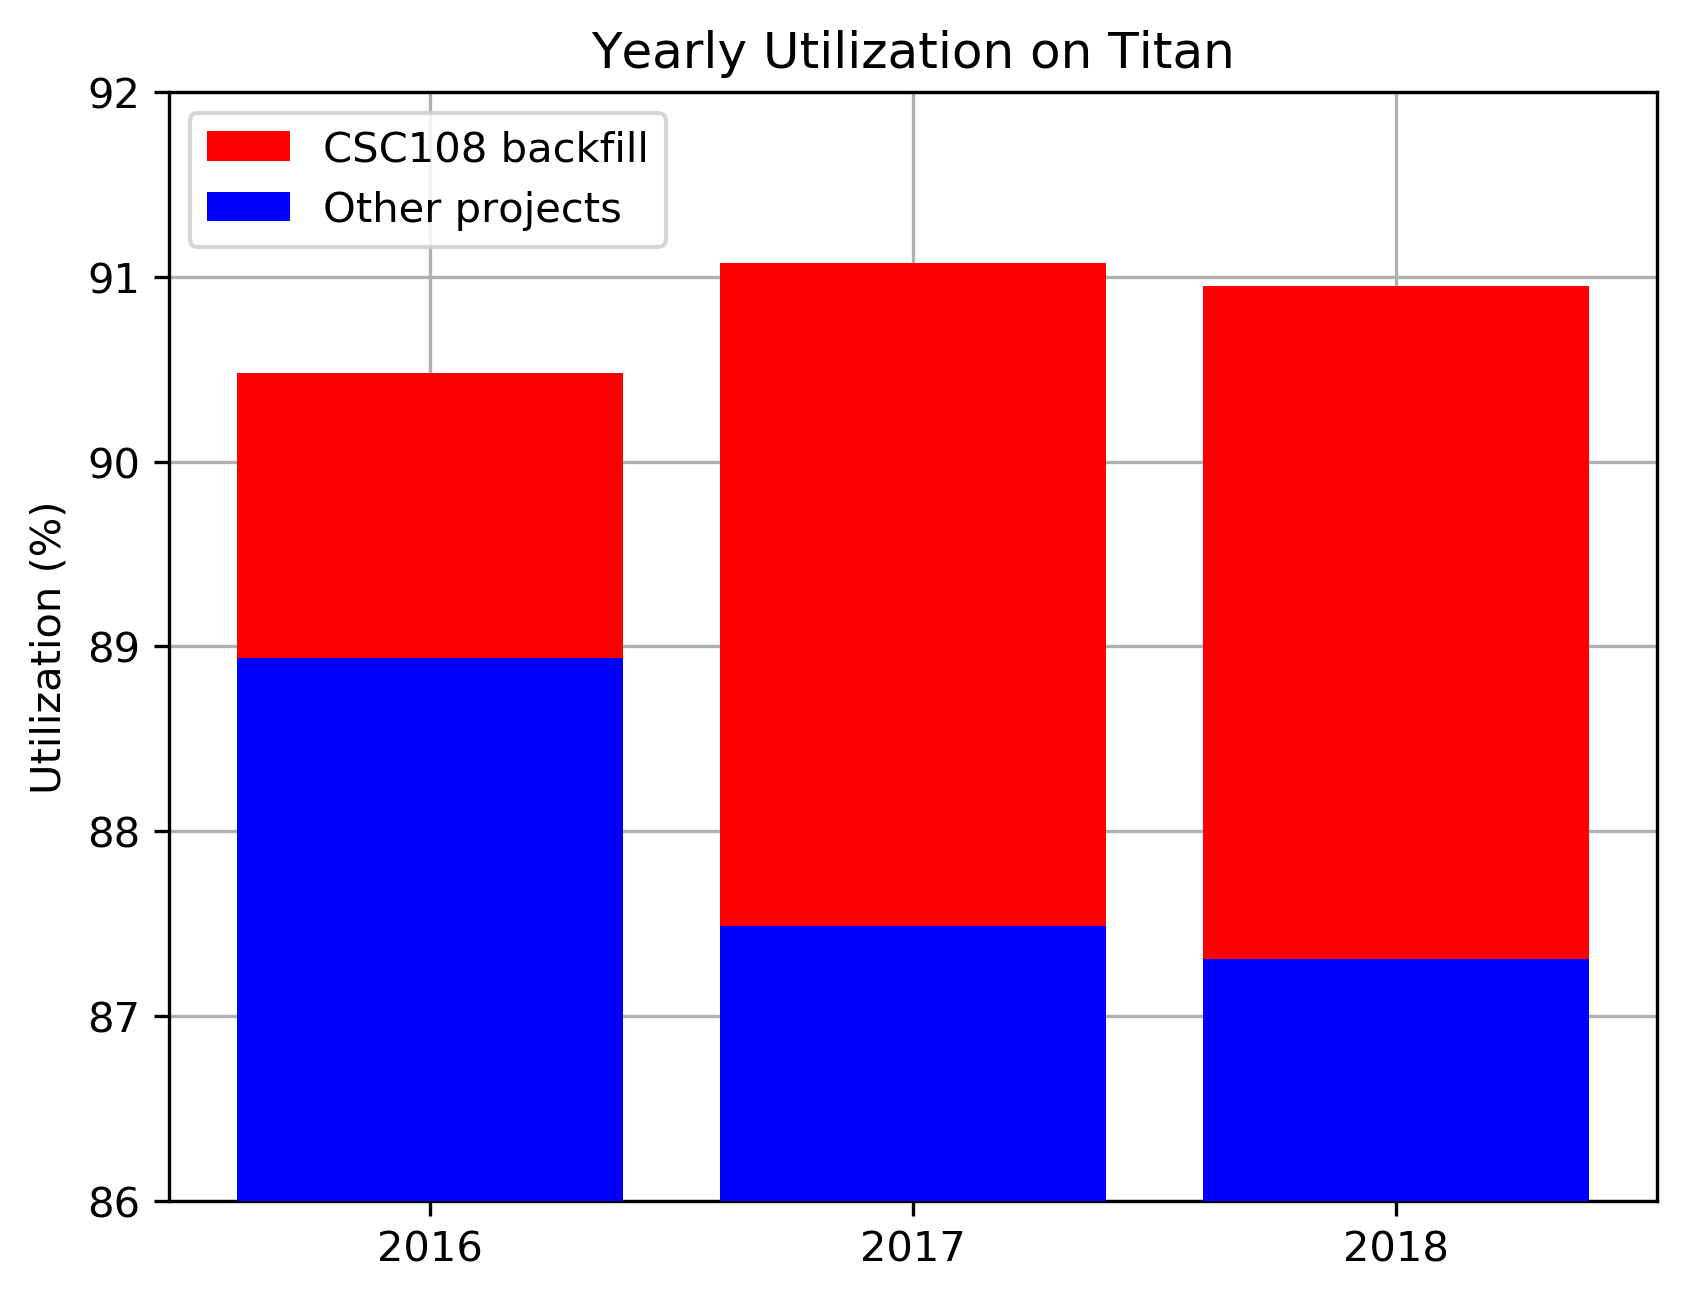
\includegraphics[width=0.75\textwidth]{images/barplot-jacks-slide.png}
% figure caption is below the figure
\caption{This bar plot visualizes the yearly utilization of Titan core hours,
separated into two categories: CSC108's utilization of Titan core hours through
backfill opportunities (shown in red), and all other utilization of core hours
on Titan (shown in blue).}
\label{fig:jacks-slide}
\end{figure*}

The data used for this experiment are historical traces for all jobs on Titan
during the years 2016, 2017, and 2018. These data were provided in anonymized
form by OLCF so that job, project, and user identifiers were included only for
the three PanDA projects on Titan. Otherwise, the job traces consist only of
job submission time, start time, completion time, the number of requested
nodes, and the amount of wall time requested. The experimental programs were
written in Python using the well-known Matplotlib, NumPy, and SciPy libraries
via Anaconda. Data were originally provided as text files but were imported
into a SQLite database. 

What we mean by ``compressing'' job traces is rescheduling the jobs that ran
on Titan while preserving the original execution order, under the assumption of
100\% availability (all nodes up and running all the time). Doing this once
while including CSC108's jobs and once with CSC108's jobs removed allows
effects on throughput and utilization to be estimated simply, using the same
logic as measuring the displacement of rocks in a jar by measuring the volume
in the jar with and without those rocks. Throughput was defined as jobs
completed per day, and utilization was defined as the percentage of available
core hours which were consumed.

The rescheduling algorithm is shown as pseudo-code in
Listing~\ref{lst:rescheduling.py}.

\lstinputlisting[language=Python,
    label={lst:rescheduling.py},
    caption={Job traces are assumed to be sorted in order of original start
                time.}]{rescheduling.py}

The results, which are shown in Table~\ref{tab:compression-results}, suggest
that the hypothesis that CSC108 has no effect on Titan should be rejected. If
CSC108 had no effect, then the percent changes in time to completion,
throughput, and utilization would all have been zero. The 1.30\% increase in
the time to completion demonstrates that CSC108's jobs displaced other
projects' jobs in this study, but the 1.94\% change in utilization indicates
that CSC108's jobs must have consumed resources which would otherwise have gone
to waste. These results suggest that CSC108 has impacted Titan both positively
and negatively in real life, and that the positive impact may justify the
negative. More importantly, however, these results suggest that CSC108 has
successfully consumed idle resources which would otherwise have gone to waste.


% For tables use
\begin{table}
% table caption is above the table
\caption{Compression study results}
\label{tab:compression-results}       % Give a unique label
% For LaTeX tables use
\begin{tabular}{lrrr}
\hline\noalign{\smallskip}
\phantom{booga}     &   Without CSC108  &   With CSC108 &   Percent change  \\
\hline\noalign{\smallskip}
Time to completion (days)           &   1021.2  &   1034.5  &   1.30        \\
Throughput (jobs per day)           &   1324.93 &   1515.19 &   14.36       \\
Utilization (percent)               &   92.36   &   94.15   &   1.94        \\
\noalign{\smallskip}\hline
\end{tabular}
\end{table}


%%%%%%%%%%%%%%%%%%%%%%%%%%%%%%%%%%%%%%%%%%%%%%%%%%%%%%%%%%%%%%%%%%%%%%%%%%%%%%%%
\subsection{Simple linear relationships}
\label{subsec:simple-linear-relationships}

% So here, I need to present a bunch of results cleverly because I never found
% any conclusive patterns.

Recall that the goal of CSC108 has been to consume idle resources on Titan
which would otherwise have gone to waste, while also making a good faith effort
not to disturb the rest of Titan's ecosystem. The results of
Section~\ref{subsec:compression-study} suggested that CSC108 has satisfied part
of this goal, but that it may have disturbed Titan's ecosystem. In this
section, we detail our explorations to understand the impact of CSC108 on Titan
and search for simple linear relationships, especially direct and inverse
relationships, by using ordinary least-squares regression.

The data used for this experiment include the same historical trace data used
in Section~\ref{subsec:compression-study}, supplemented with daily availability
data for Titan provided by OLCF for the same years, 2016-2018. The experimental
programs were written in Python using the well-known Matplotlib, NumPy, SciPy,
and scikit-learn libraries via Anaconda. Data were originally provided as text
files but were imported into a SQLite database. We plotted best-fit lines with
ordinary least squares (OLS) linear regression, constructed 95\% confidence
regions around the lines, and used basic measures for goodness-of-fit such as
R-squared.

There were two main ideas used here. The first idea was to look for a
relationship between CSC108's throughput and the throughput of all other jobs
on Titan, and second idea was to look for a relationship between CSC108's
utilization as compared with overall utilization on Titan. Additionally, the
same ideas were repeated to look for impacts due to different sizes of CSC108's
jobs, using the bins defined in Table~\ref{tab:olcf-bins}, because jobs are
assigned priority differently by the scheduler on Titan in part due to the
number of requested nodes and length of requested wall time.

%%%
% THROUGHPUT FIGURES AS SUBFIGURES
%%%
\begin{figure*}
  \subfloat[All\label{fig:throughput-all}]{
    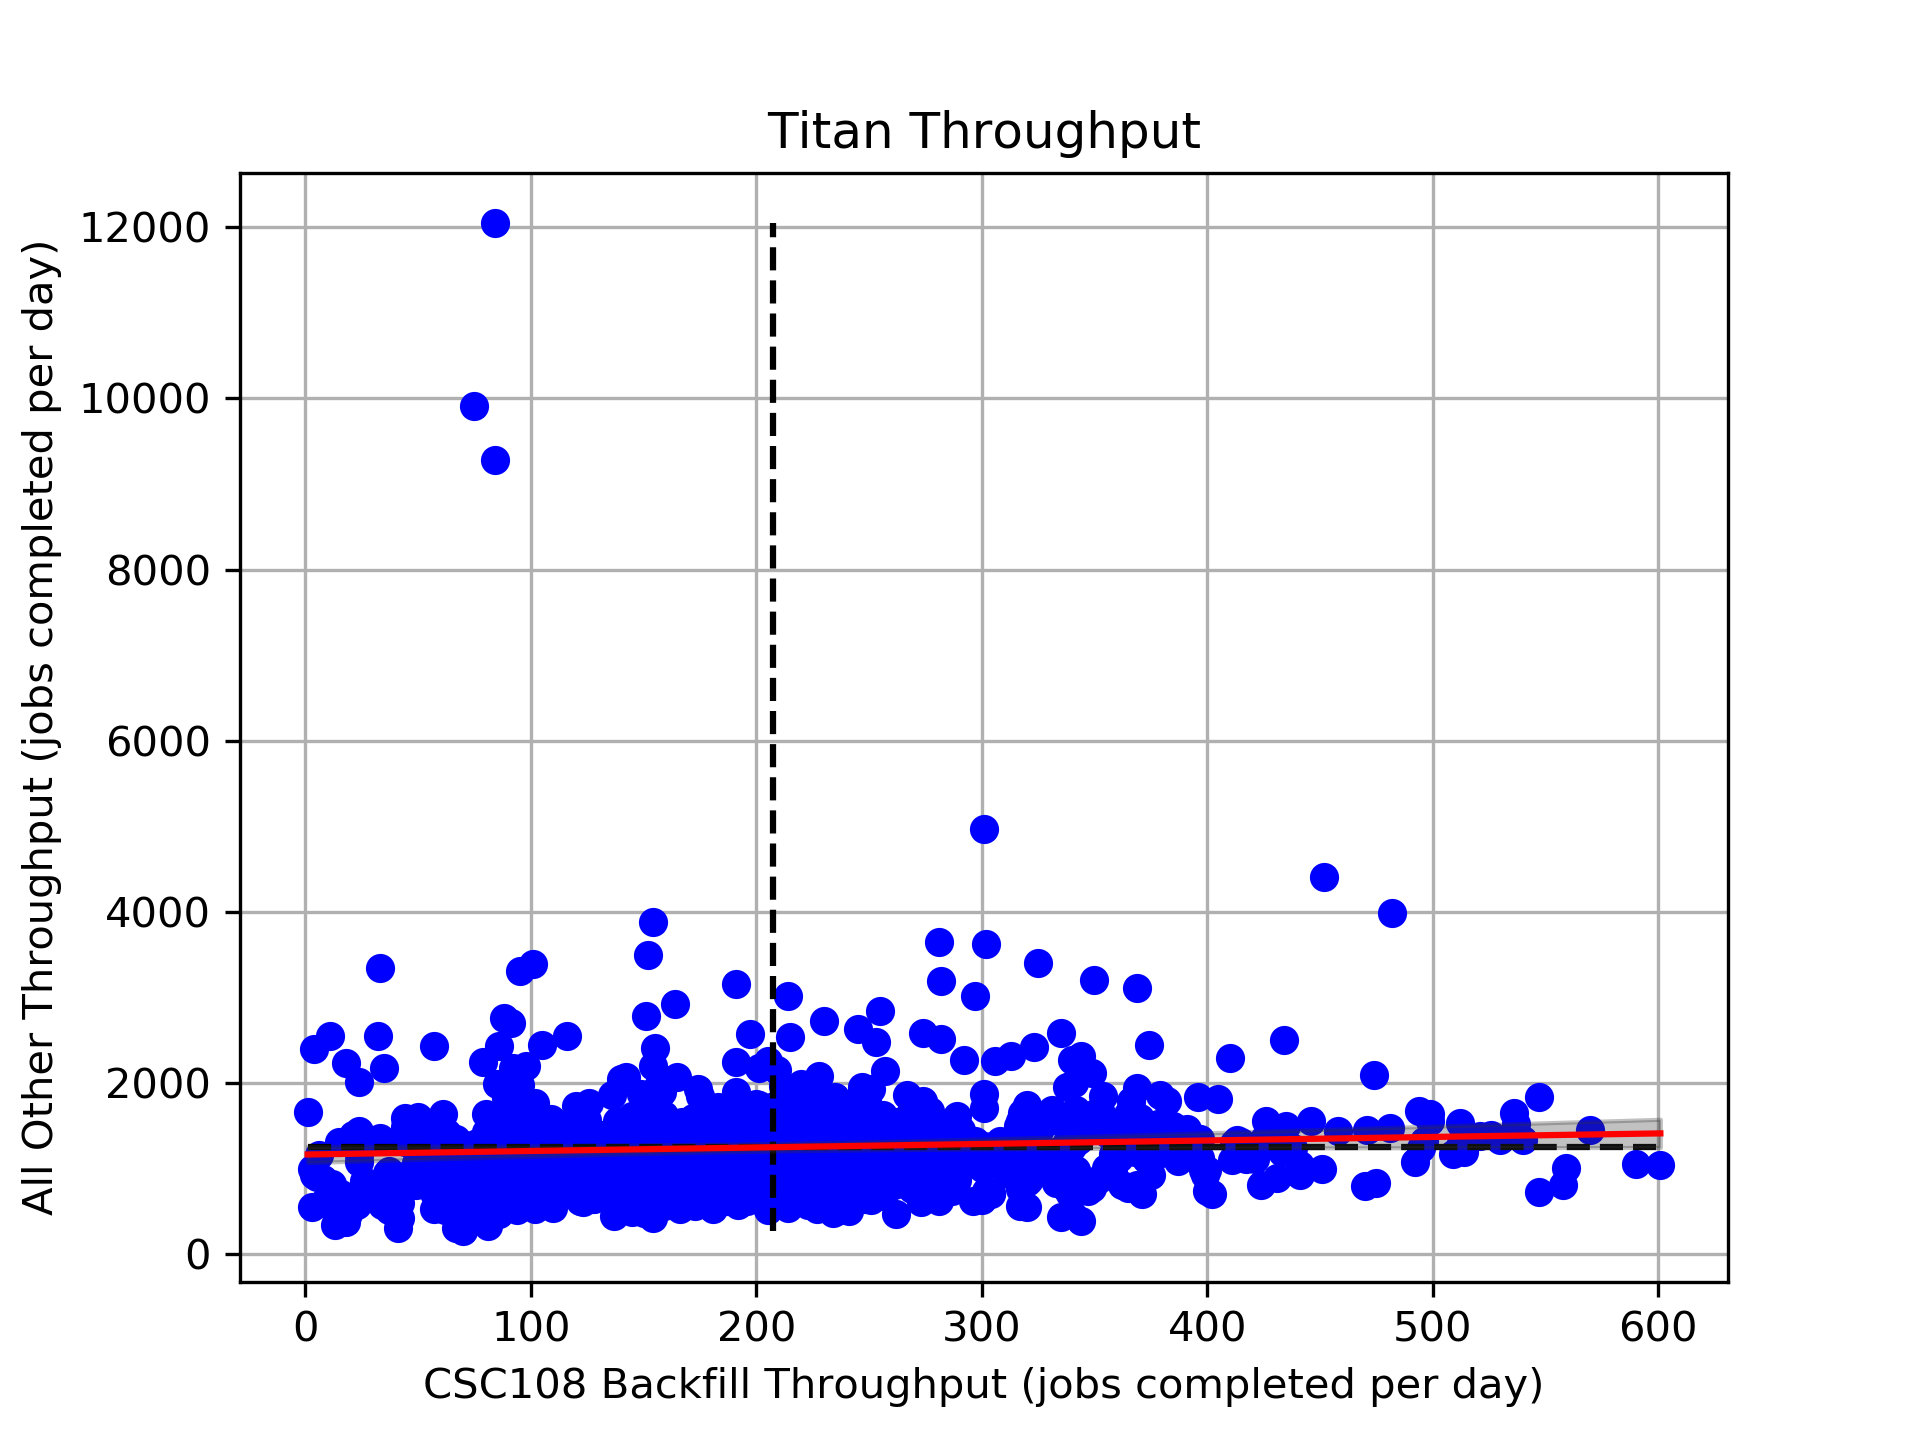
\includegraphics[width=0.4\textwidth]{images/linfit-throughput-all.png}}
  \subfloat[Bin 3\label{fig:throughput-bin3}]{
    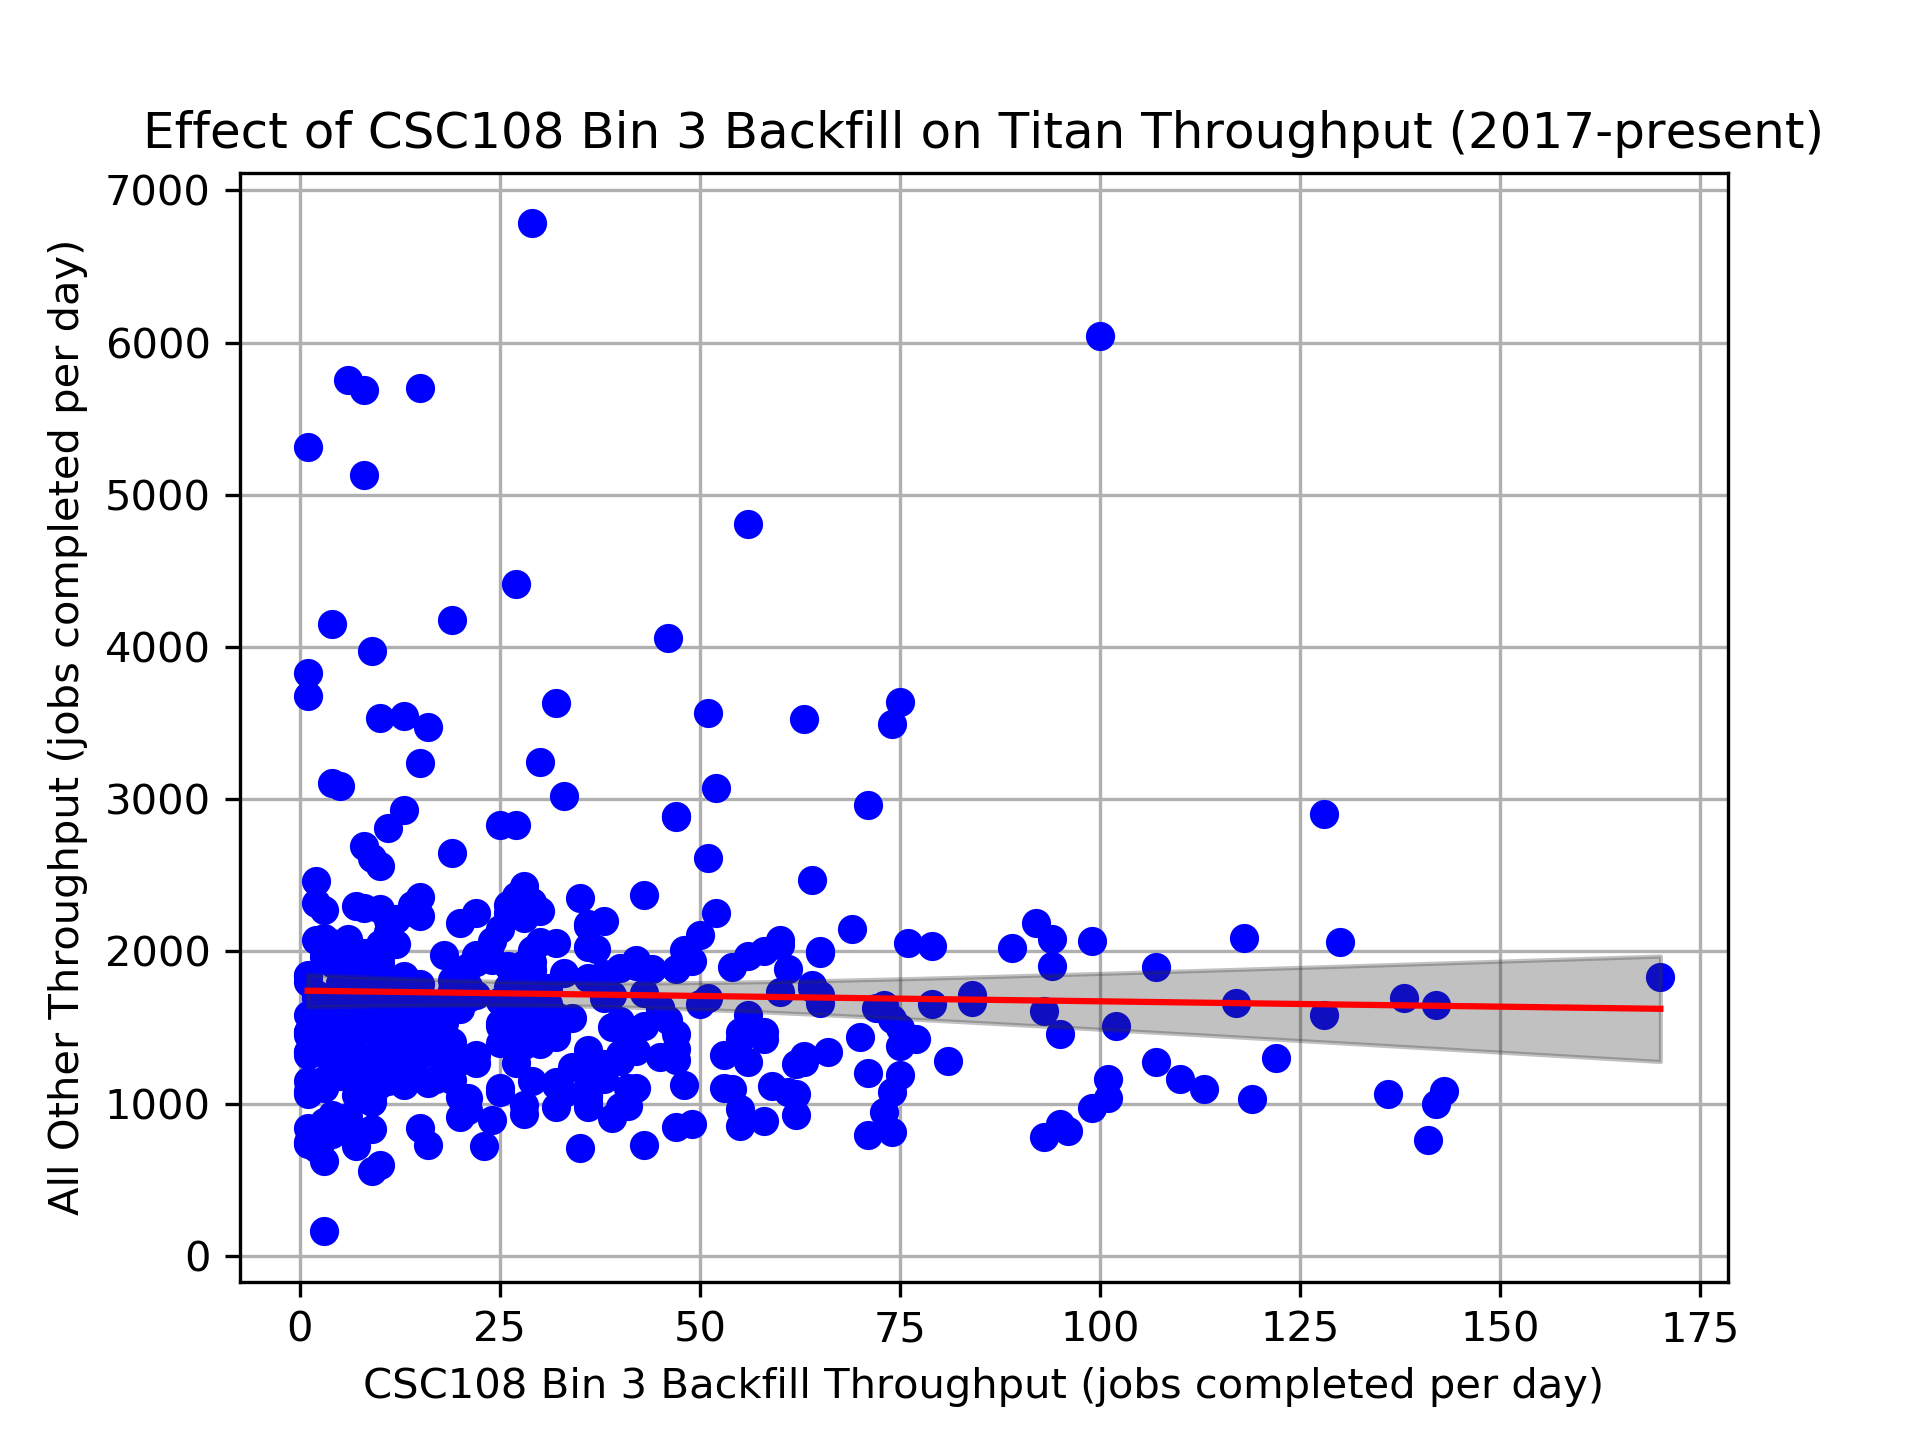
\includegraphics[width=0.4\textwidth]{images/linfit-throughput-bin3.png}}
  \vspace{1em}
  \subfloat[Bin 4\label{fig:throughput-bin4}]{
    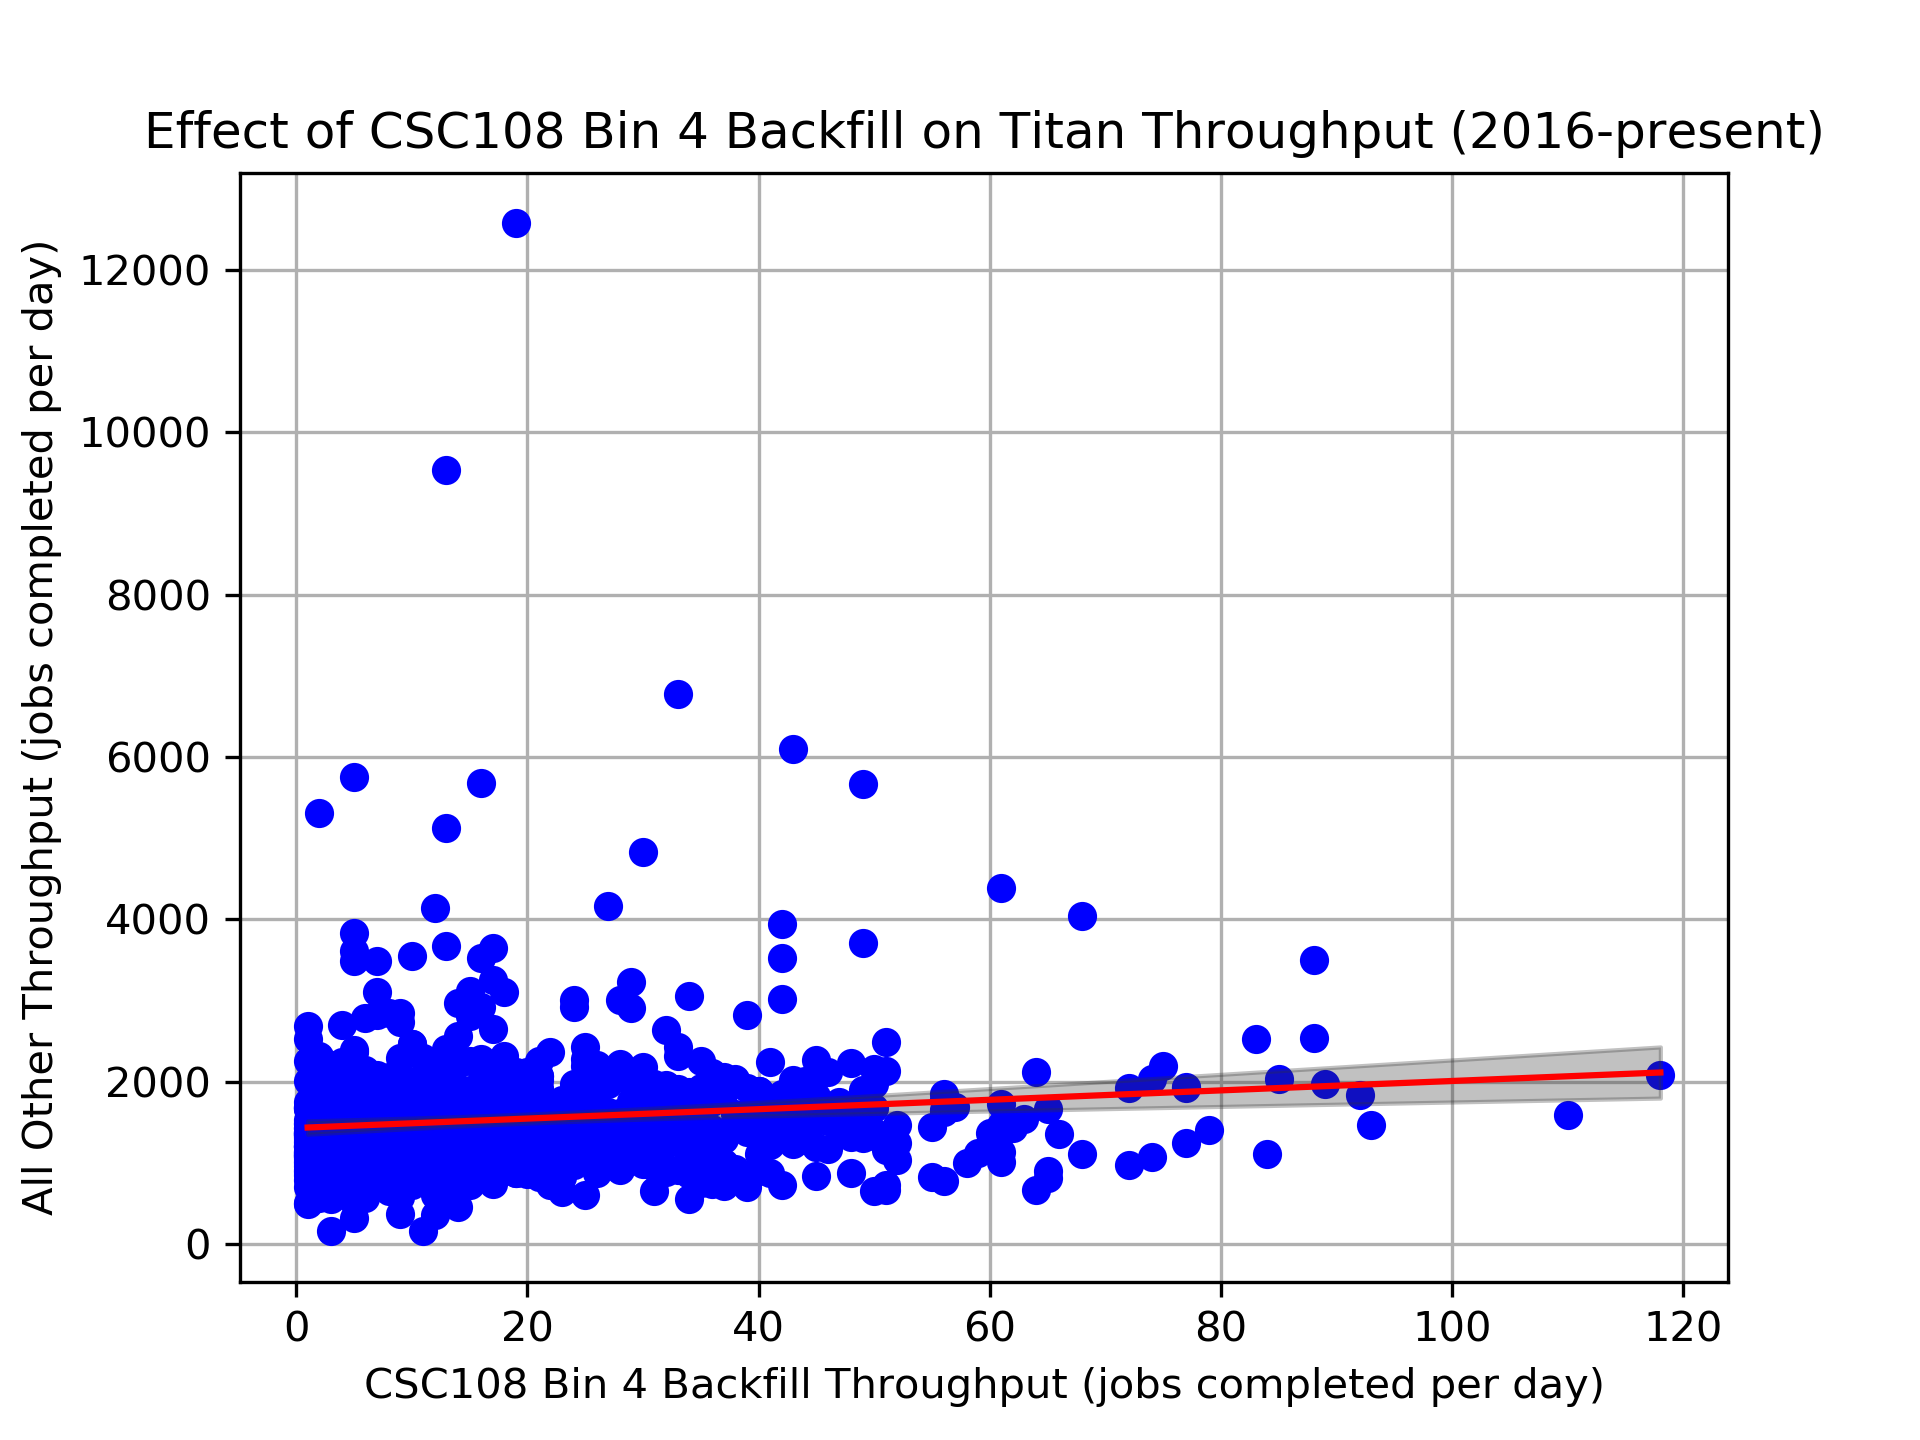
\includegraphics[width=0.4\textwidth]{images/linfit-throughput-bin4.png}}
  \subfloat[Bin 5\label{fig:throughput-bin5}]{
    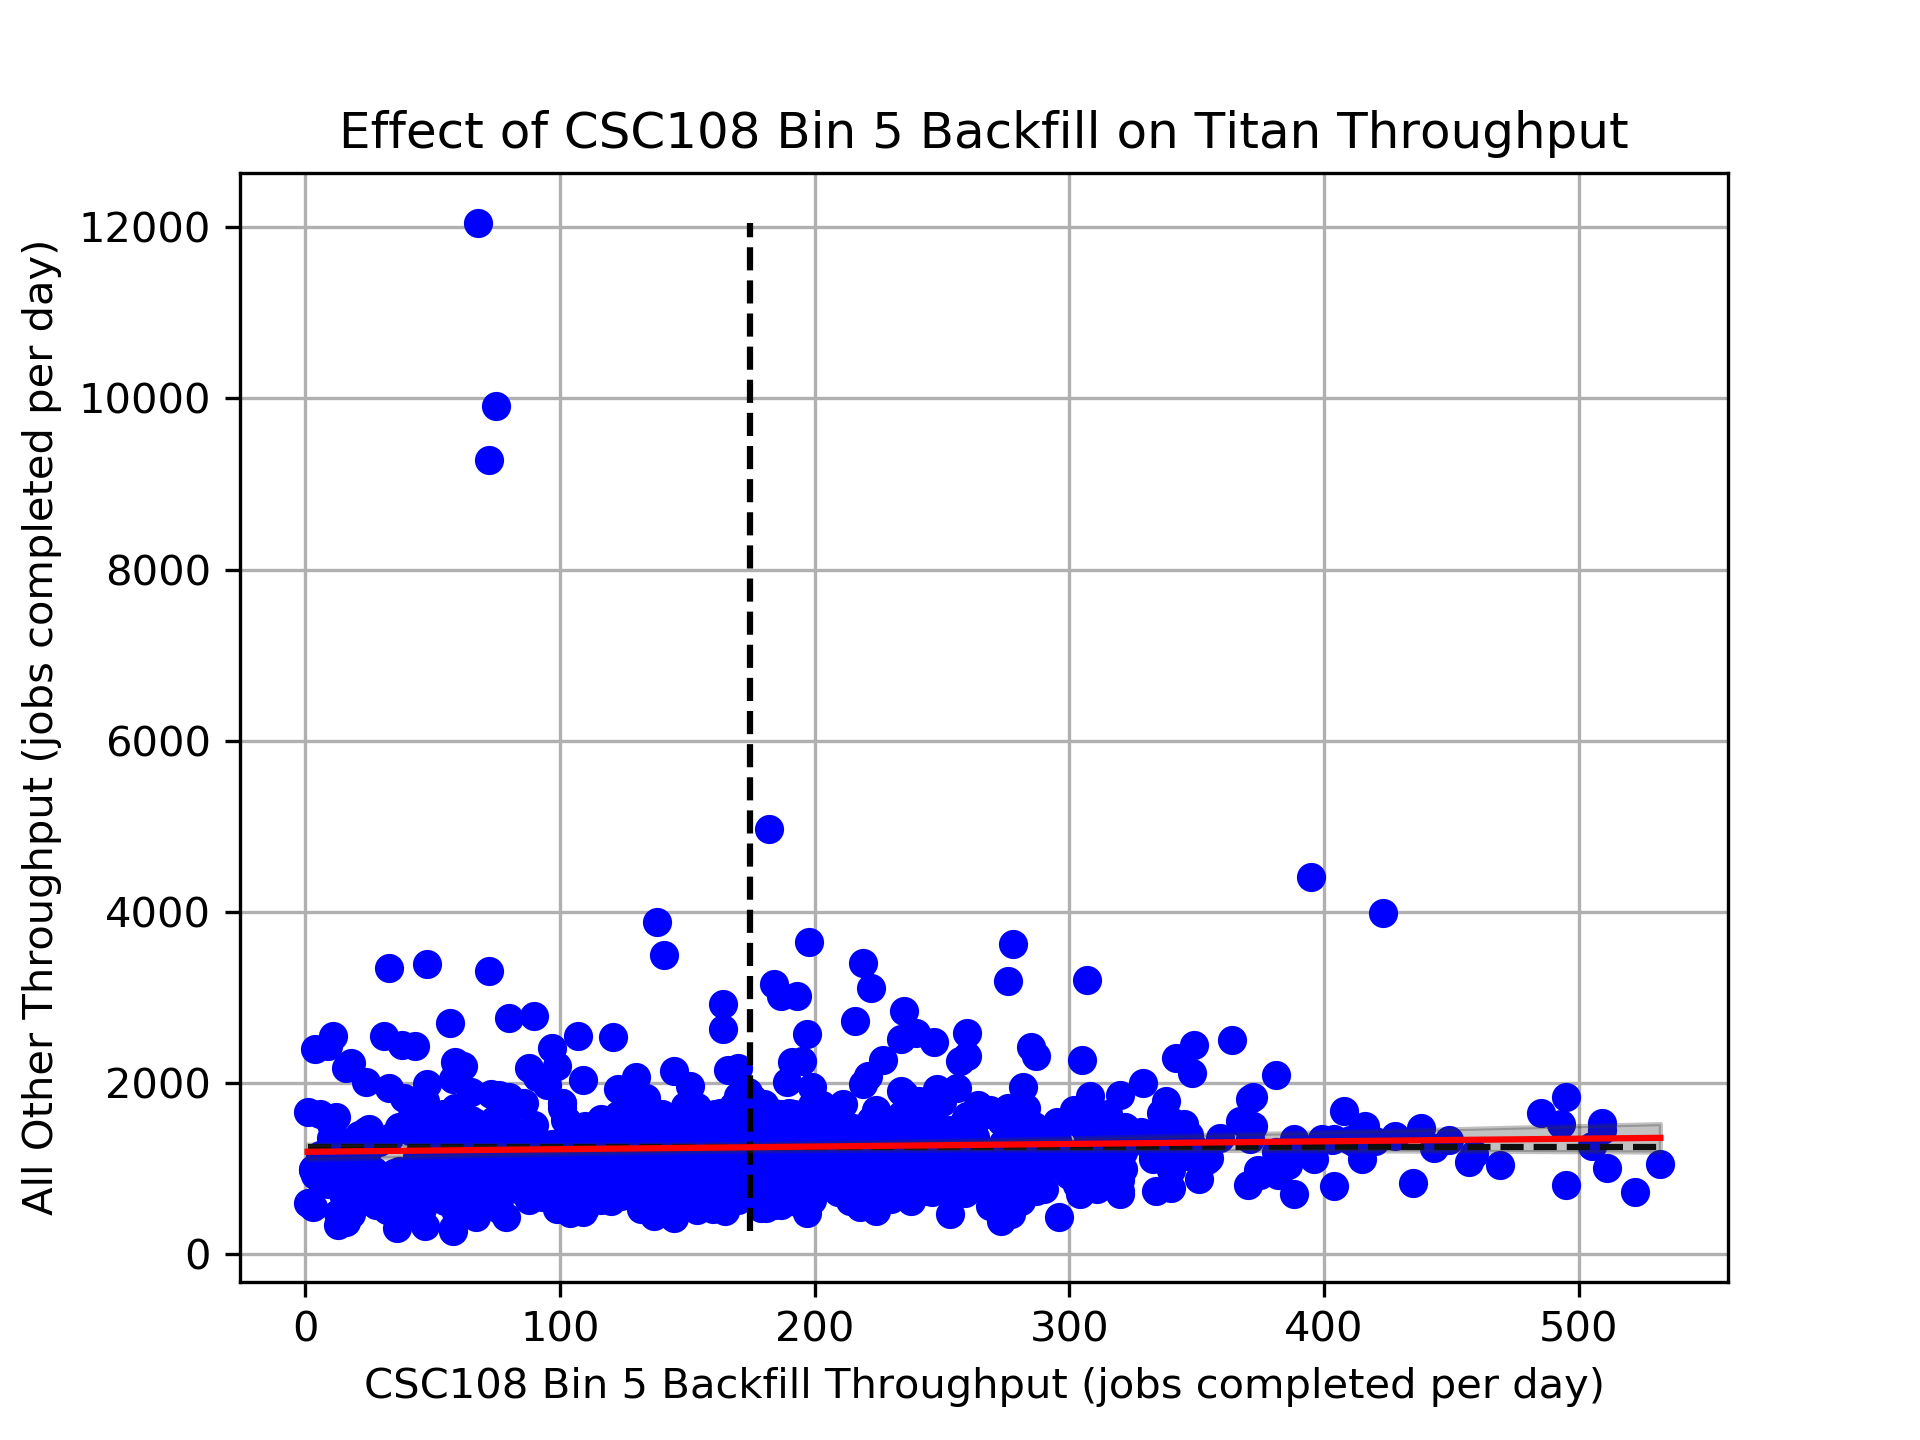
\includegraphics[width=0.4\textwidth]{images/linfit-throughput-bin5.png}}
  \caption{This figure demonstrates the relationship between CSC108 backfill
throughput and throughput of other projects on Titan, in terms of jobs
completed per day. Each blue point represents one day. Each red line is an
Ordinary Least Squares (OLS) linear regression with parameters given in
Table~\ref{tab:throughput-params}. Each shaded gray area represents a 95\%
confidence region. Each horizontal dotted black line represents the mean number
of jobs completed on Titan every day by projects other than CSC108, and the
vertical dotted black line represents the mean number of jobs completed every
day by CSC108's use of backfill opportunity.}
\end{figure*}

% For tables use
\begin{table}
% table caption is above the table
\caption{The table contains the parameter values for the Ordinary Least Squares
(OLS) linear regression models regarding throughput. The first column
corresponds to the figure depicting the model, and the second column
corresponds to the OLCF bin number, as defined in Table~\ref{tab:olcf-bins}.
The second and third columns correspond the coefficients $\beta_1$ and
$\beta_0$ in the model $y = \beta_{1}x + \beta_0$.}
\label{tab:throughput-params}       % Give a unique label
% For LaTeX tables use
\begin{tabular}{ccrrr}
\hline\noalign{\smallskip}
Figure & OLCF Bin & Slope $\beta_1$  & Intercept $\beta_0$  &   $\text{R}^2$ \\
\noalign{\smallskip}\hline\noalign{\smallskip}
\ref{fig:throughput-all}    &   All &   0.4106  &   1164.2561   & 0.0040    \\
\ref{fig:throughput-bin3}   &   3   &   0.4419  &   1322.0784   & 0.0005    \\
\ref{fig:throughput-bin4}   &   4   &   1.9819  &   1211.3384   & 0.0027    \\
\ref{fig:throughput-bin5}   &   5   &   0.3072  &   1195.6684   & 0.0018    \\
\noalign{\smallskip}\hline
\end{tabular}
\end{table}
%%%

%%%
% UTILIZATION FIGURES AS SUBFIGURES
%%%
\begin{figure*}
  \subfloat[All\label{fig:utilization-all}]{
    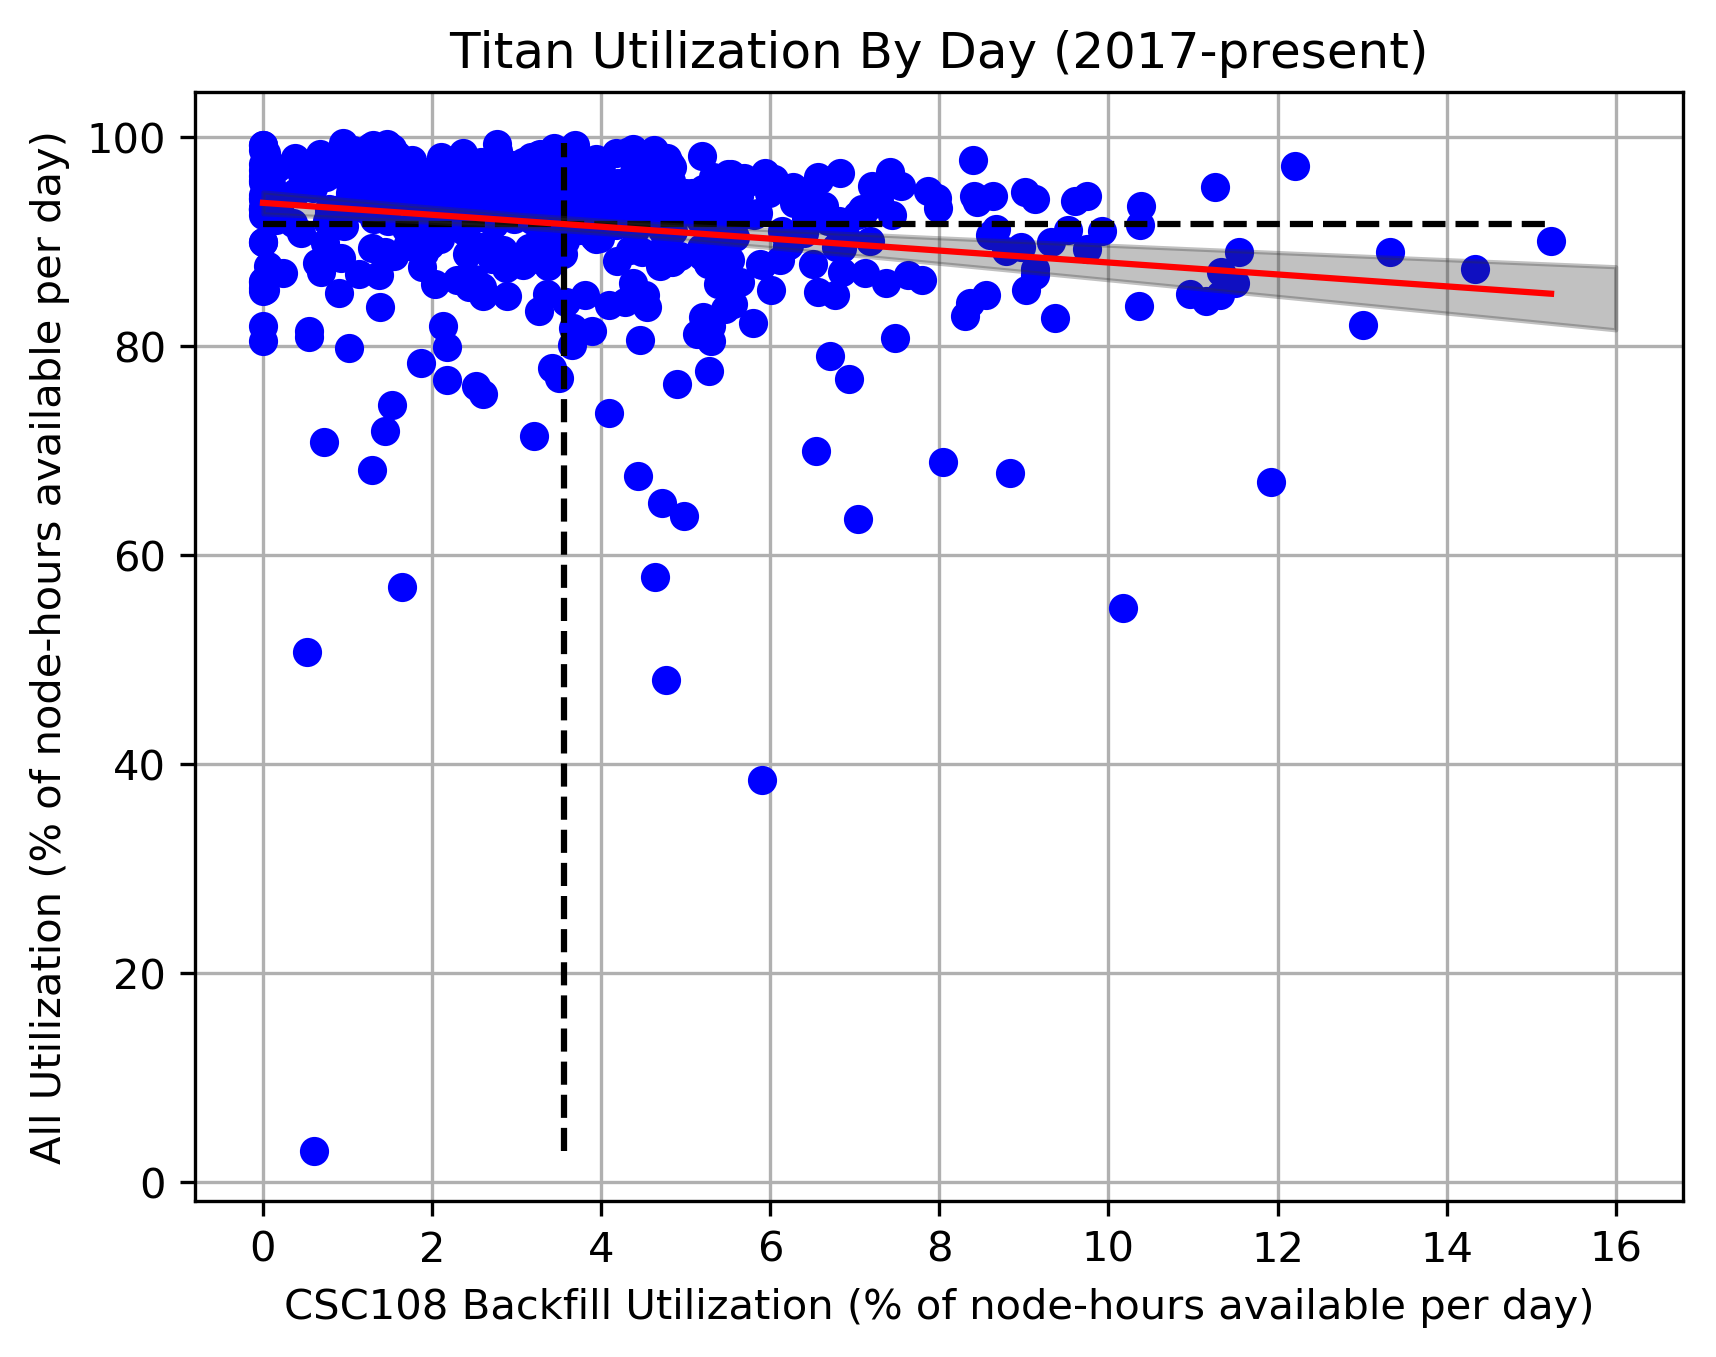
\includegraphics[width=0.4\textwidth]{images/linfit-utilization-by-true-day-all.png}}
  \subfloat[Bin 3\label{fig:utilization-bin3}]{
    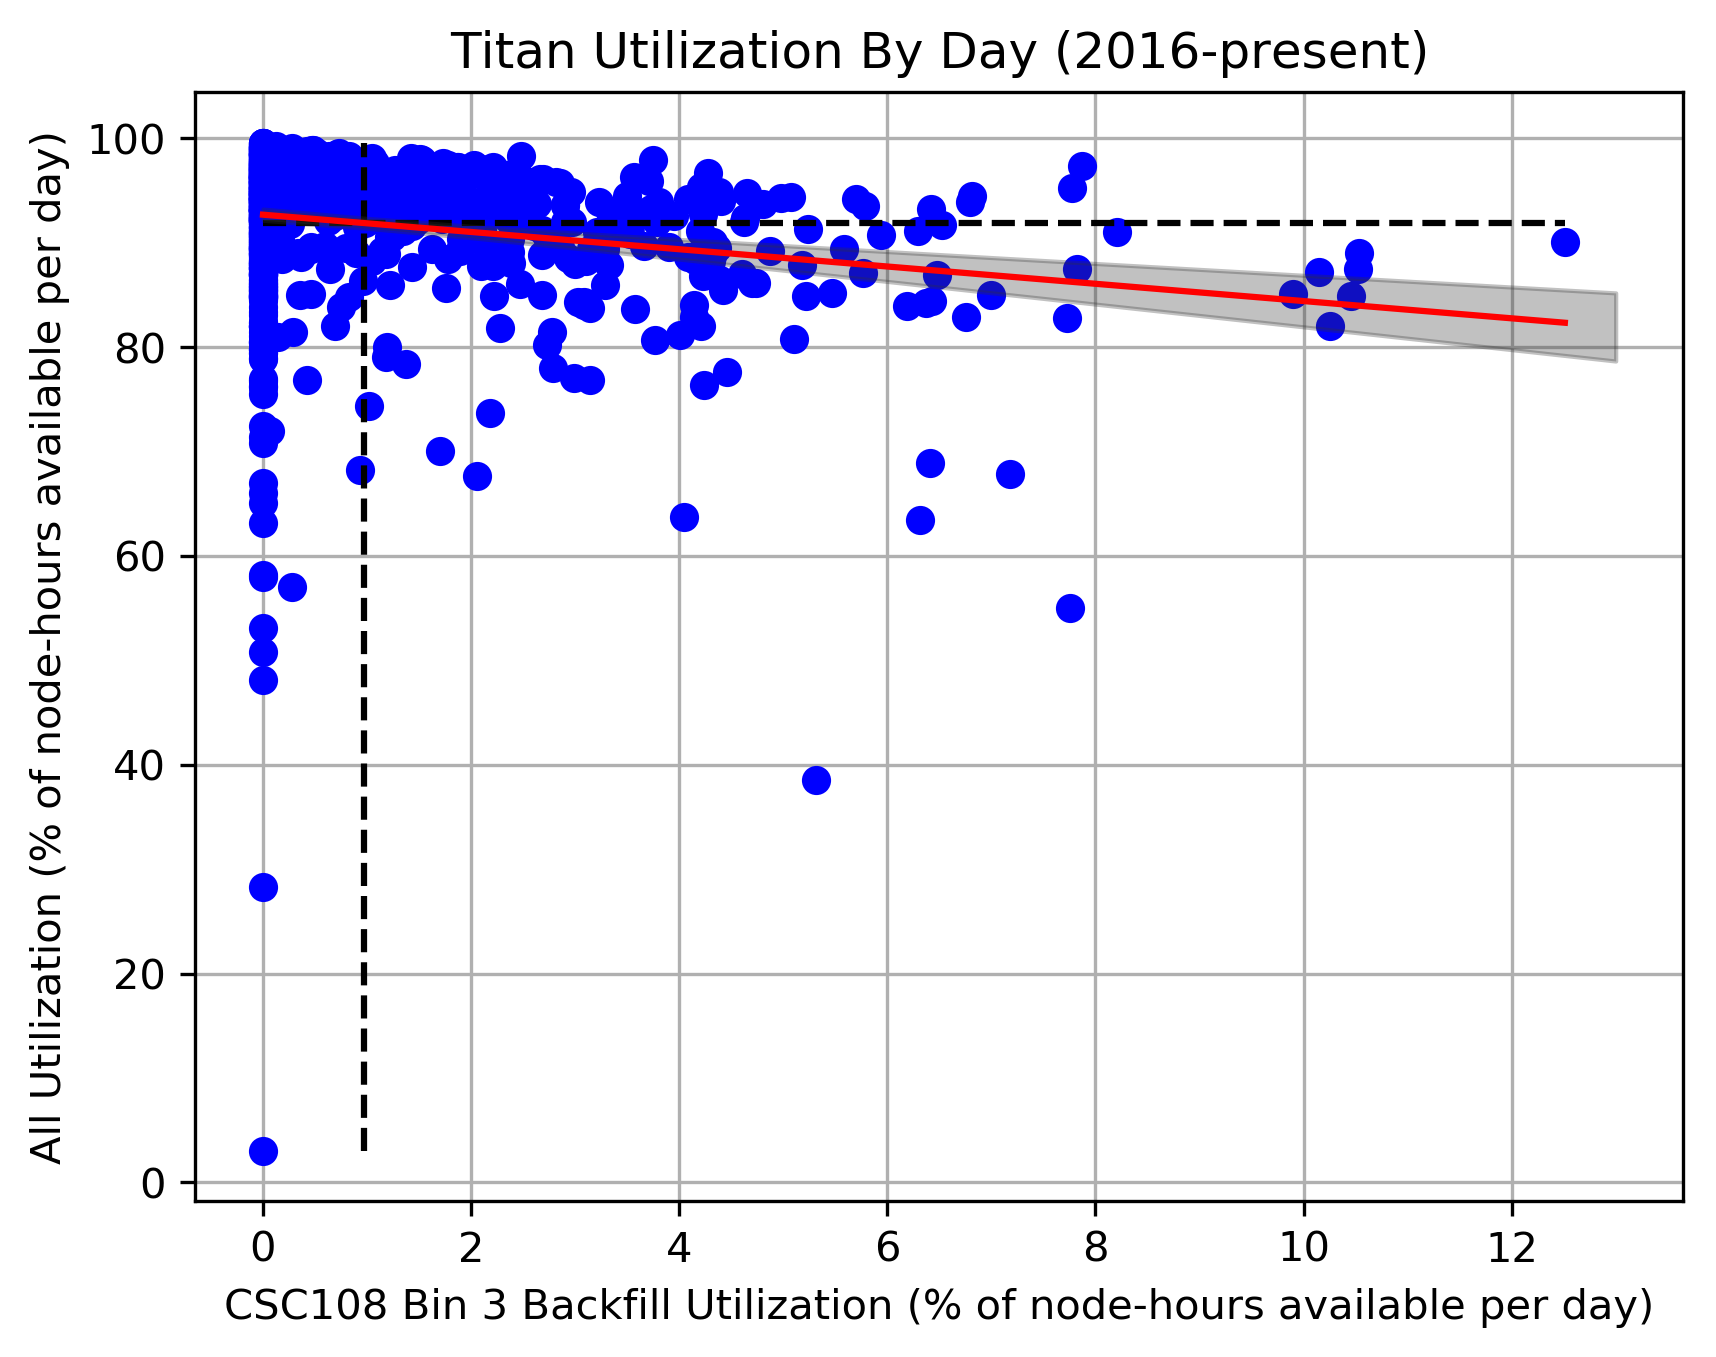
\includegraphics[width=0.4\textwidth]{images/linfit-utilization-by-true-day-bin3.png}}
  \vspace{1em}
  \subfloat[Bin 4\label{fig:utilization-bin4}]{
    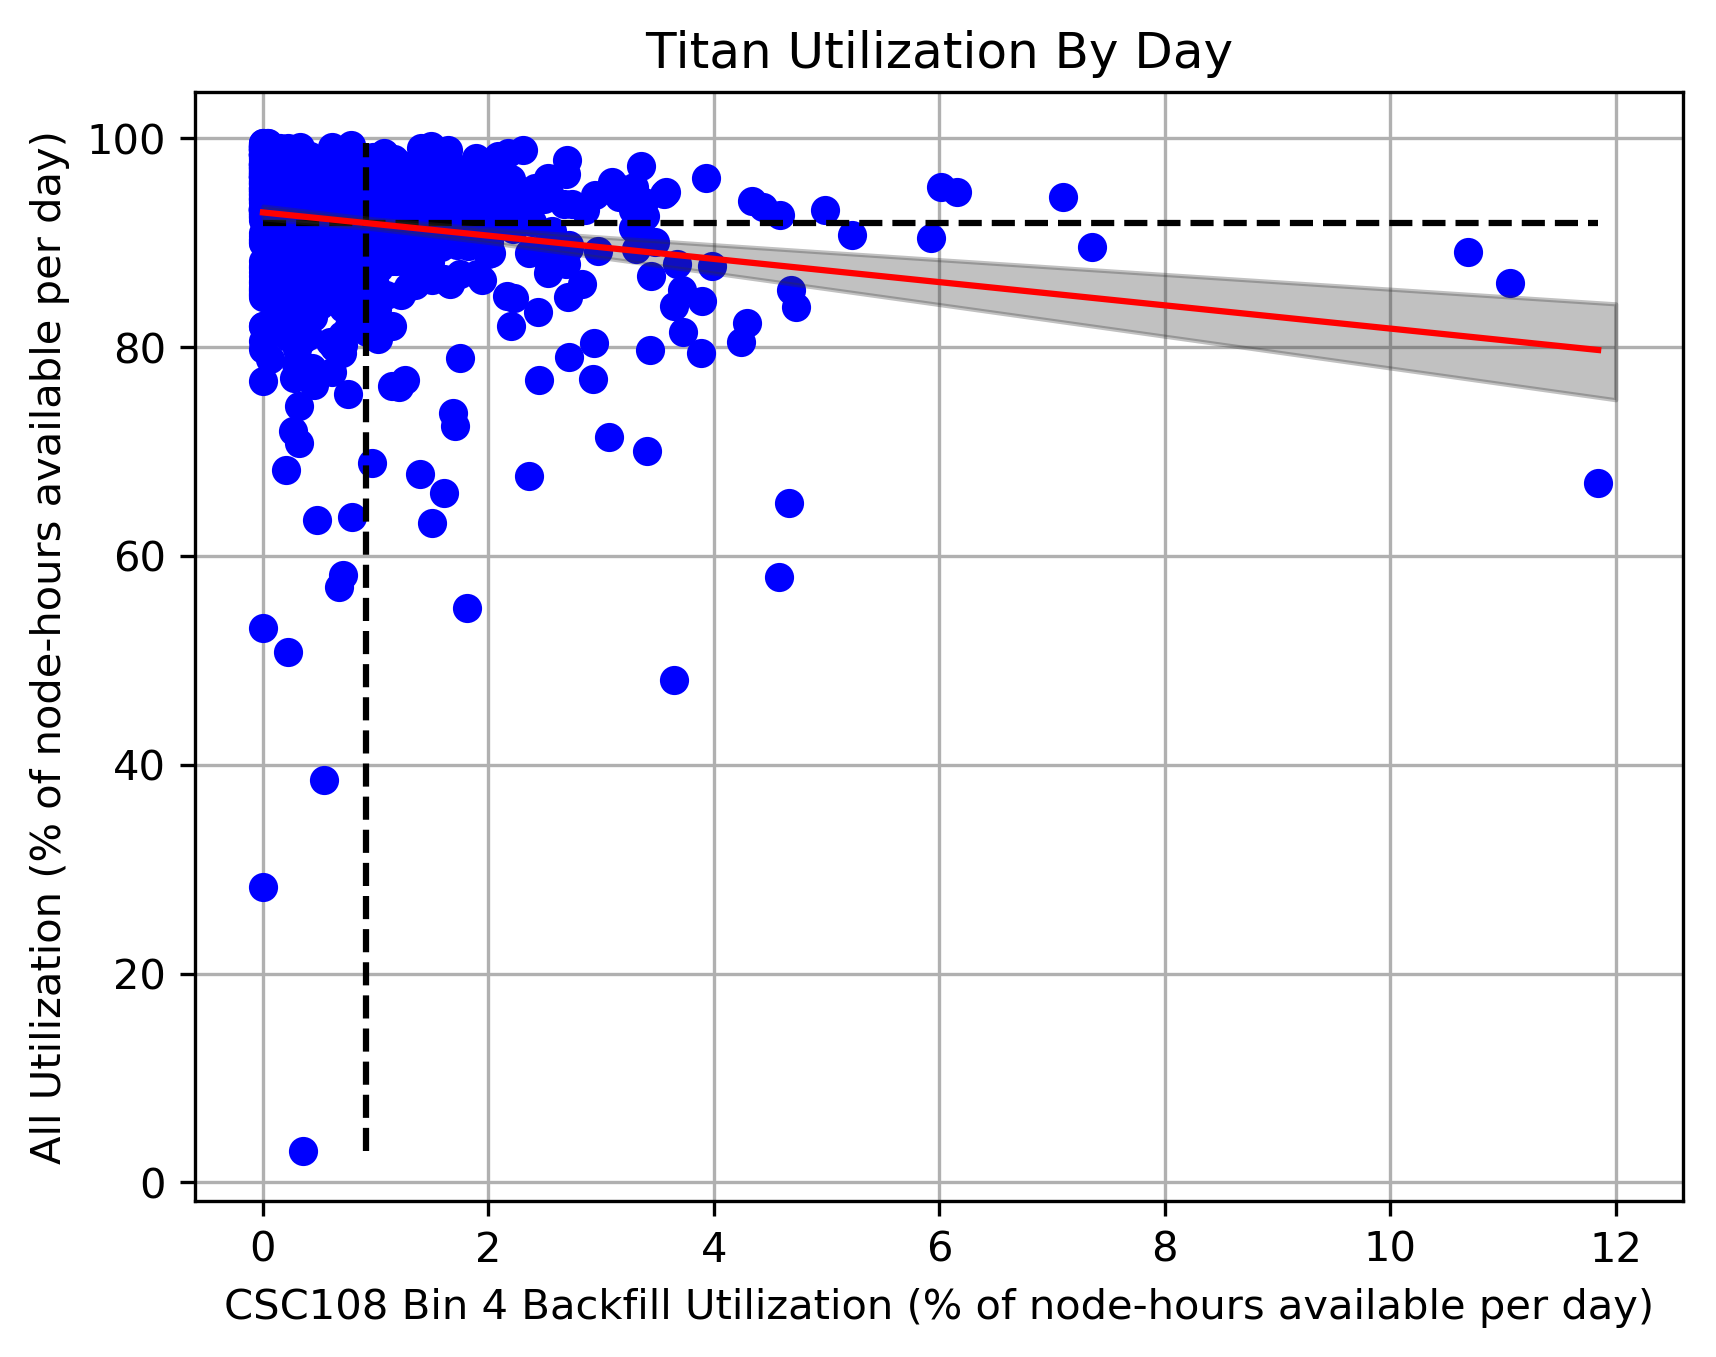
\includegraphics[width=0.4\textwidth]{images/linfit-utilization-by-true-day-bin4.png}}
  \subfloat[Bin 5\label{fig:utilization-bin5}]{
    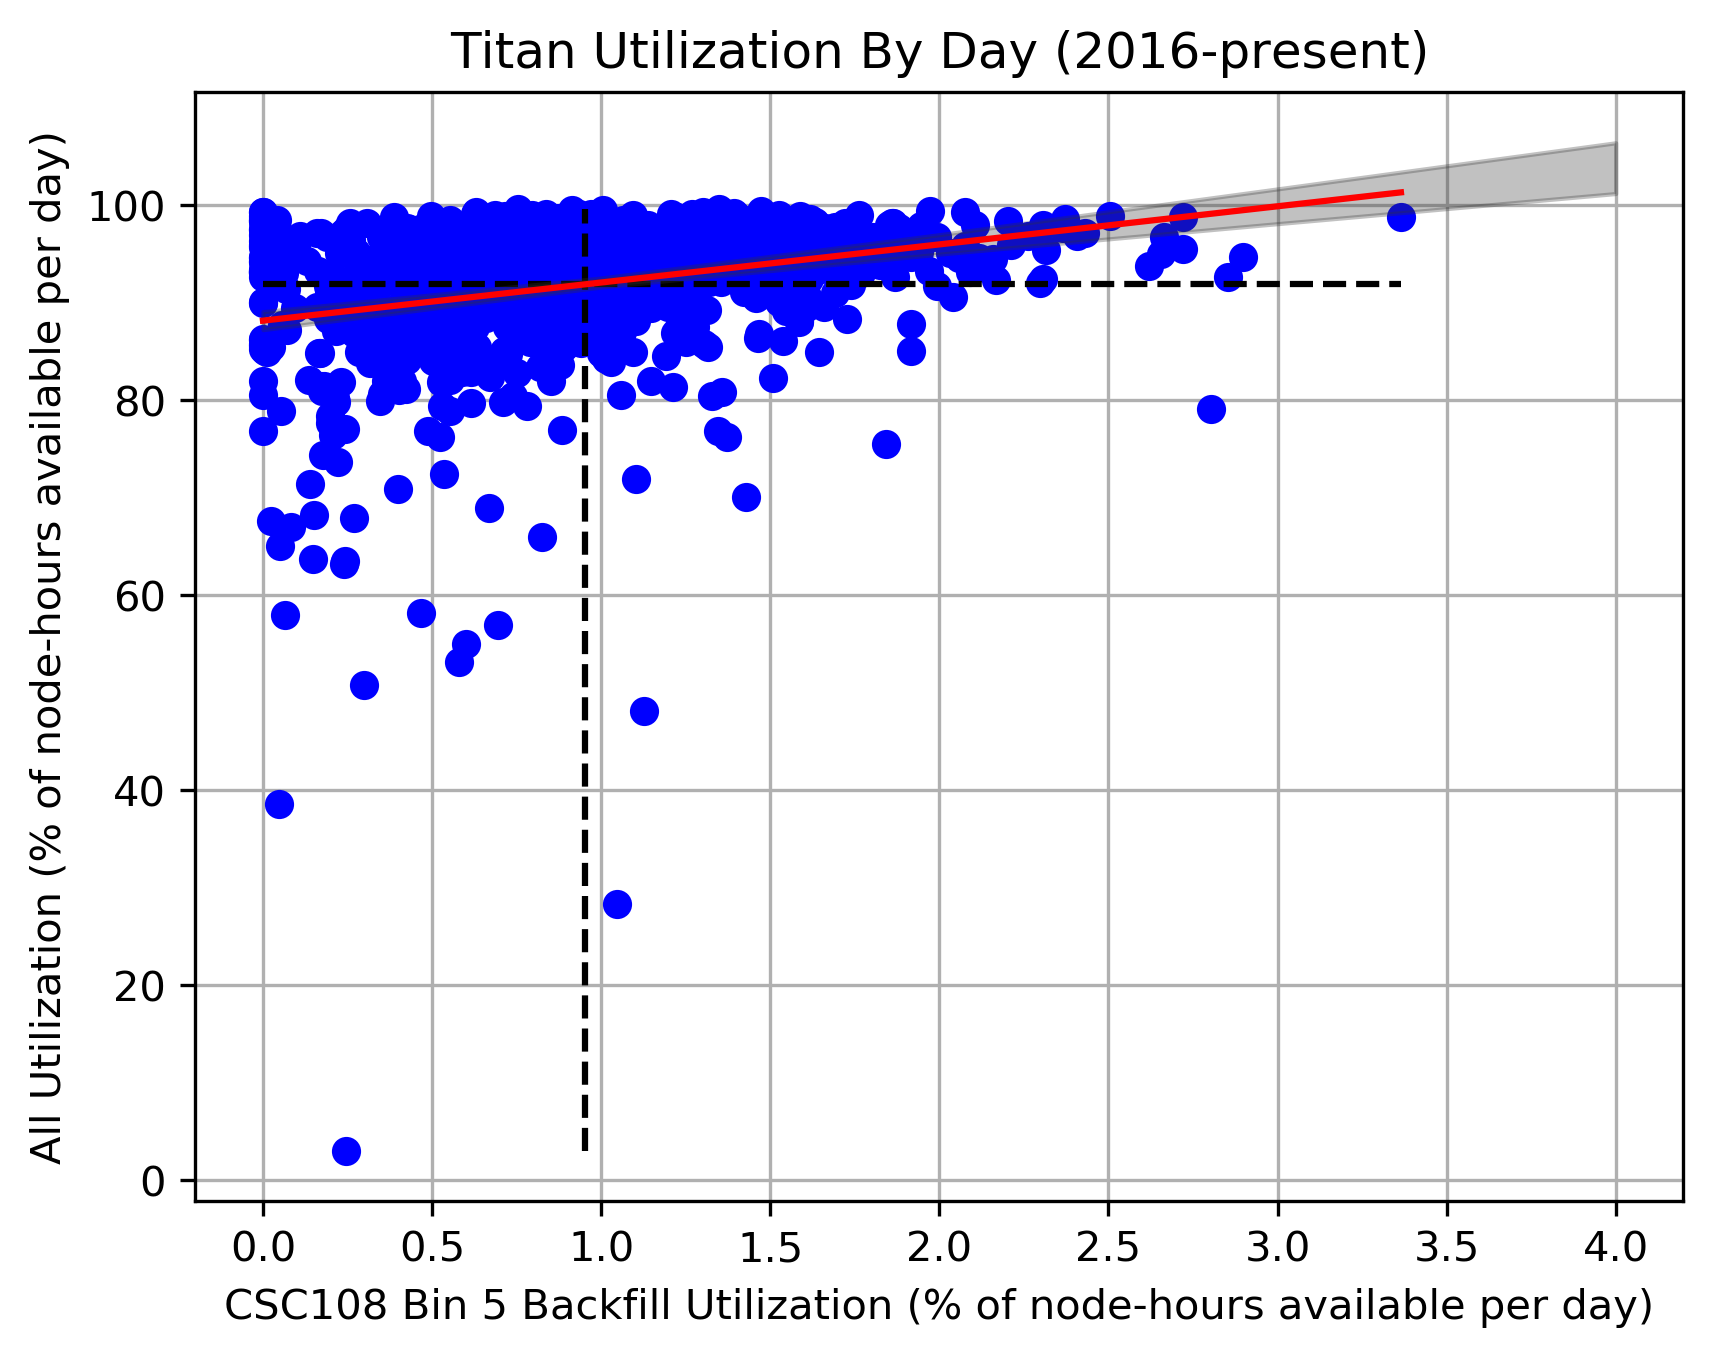
\includegraphics[width=0.4\textwidth]{images/linfit-utilization-by-true-day-bin5.png}}
  \caption{This figure demonstrates the relationship between CSC108 backfill
utilization and overall utilization on Titan, as percentages of available
node-hours each day. Each blue point represents one day. Each red line is an
Ordinary Least Squares (OLS) linear regression with parameters given in
Table~\ref{tab:utilization-params}. Each shaded gray area represents a 95\%
confidence regions. Each horizontal dotted black line represents the mean
utilization every day on Titan, and each vertical dotted black line represents
the mean utilization of backfill opportunity every day by CSC108.}
\end{figure*}

% For tables use
\begin{table}
% table caption is above the table
\caption{The table contains the parameter values for the Ordinary Least Squares
(OLS) linear regression models regarding utilization. The first column
corresponds to the figure depicting the model, and the second column
corresponds to the OLCF bin number, as defined in Table~\ref{tab:olcf-bins}.
The second and third columns correspond the coefficients $\beta_1$ and
$\beta_0$ in the model $y = \beta_{1}x + \beta_0$.}
\label{tab:utilization-params}       % Give a unique label
% For LaTeX tables use
\begin{tabular}{ccrrr}
\hline\noalign{\smallskip}
Figure  & OLCF Bin & Slope $\beta_1$  & Intercept $\beta_0$  &  $\text{R}^2$ \\
\noalign{\smallskip}\hline\noalign{\smallskip}
\ref{fig:utilization-all}    &   All &  -0.5258 &   93.3404     &   0.0330  \\
\ref{fig:utilization-bin3}   &   3   &  -1.0977 &   94.0609     &   0.1359  \\
\ref{fig:utilization-bin4}   &   4   &  -1.1472 &   92.7870     &   0.0378  \\
\ref{fig:utilization-bin5}   &   5   &   4.3328 &   87.5839     &   0.1046  \\
\noalign{\smallskip}\hline
\end{tabular}
\end{table}
%%%

The plots shown in Figures~\ref{fig:throughput-all}, \ref{fig:throughput-bin3},
\ref{fig:throughput-bin4}, and \ref{fig:throughput-bin5} visually suggest that
CSC108 has little to no effect on other projects' throughputs, but the numbers
in Table~\ref{tab:throughput-params} show that linear relationships explain
very little of the variability in the data. The $\text{R}^2$ values, which
represent goodness-of-fit on a scale of 0 to 1, are very close to 0, indicating
poor fit.

Similar problems exist for the utilization results, but they raise one very
interesting question. The plots shown in Figures~\ref{fig:utilization-all},
\ref{fig:utilization-bin3}, and \ref{fig:utilization-bin4} all clearly suggest
an inverse relationship, but \ref{fig:utilization-bin5} suggests a direct
relationship, by virtue of its positive slope. Unfortunately, once again, the
numbers show that linear relationships explain very little of the variability
in the data, as shown in Table~\ref{tab:utilization-params}, because the
$\text{R}^2$ values are very close to 0, on a scale of 0 to 1. This raises the
question, what has caused the sign change? It can be tempting to assign blame
and credit in such a case, such as to say that CSC108's consumption in bin 5
causes an increase in overall utilization, while its consumption in other bins
decreases overall utilization. Here, however, we are only looking for
relationships in the data, and the goodness-of-fit values are uniformly poor. 


%%%%%%%%%%%%%%%%%%%%%%%%%%%%%%%%%%%%%%%%%%%%%%%%%%%%%%%%%%%%%%%%%%%%%%%%%%%%%%%%
\subsection{Blocking probability}
\label{subsec:blocking-probability}

Having struggled to find simple linear relationships using throughput and
utilization as indicators, we next defined an event called a ``block'' and
looked for its occurrence in the data. A block is said to occur when an
eligible job in the batch queue waits due to insufficient resources on Titan
for it to begin running; some other job(s) must be using the resources, and
therefore the eligible job has been ``blocked'' by an already-running job. This
event is interesting because it can indicate competition for resources even
when there are large amounts of idle resources. It also serves as a way to
symbolize the event when a user checks the system queue and sees that there are
active jobs that are causing the user's job to wait. The goal was to try to
detect CSC108's impact by focusing on times of great competition.

The data used for this experiment include the same historical trace data used
in Section~\ref{subsec:compression-study} and the daily availability
data for Titan used in Section~\ref{subsec:simple-linear-relationships}, but
this time are supplemented with live snapshot data of the system queue for
Titan. Snapshots were gathered by sampling live data from the Moab scheduler by
polling with Python scripts launched by cron jobs on a data transfer node.
These scripts recorded XML output from the ``showbf'' and ``showq'' commands
into files, and more cron jobs launched other Python scripts to import these
files' sample data into SQLite. These tables contain data about the exact state
of the queues at given times, including active jobs, blocked jobs, eligible
jobs, recently completed jobs, and system information such as active nodes and
available backfill opportunities. Then, experimental programs were written in
Python using the same libraries and database as the previous sections.

Formally, the definitions for a block and a blocking probability follow. Let
$C_i$ be the abstract resources in use by CSC108 at the $i^{\text{th}}$ sample
point in time, and let $U_i$ be the unused (idle) resources remaining on Titan.
We then define a boolean $B_i$ representing a ``block'' to be 1 if there exists
at least one job at the $i^{\text{th}}$ sample point which requests
$(C_i + U_i)$ resources or less when $C_i$ is non-zero; we define $B_i$ to be
zero otherwise. Summing $B_i$ over all $i$ gives a count of sample points at
which a block occurred, and dividing that count by the number of total sample
points yields a quantity we call a ``blocking probability''. The blocking
probability is a rational number between 0 and 1.

Informally, blocking probability represents the proportion of samples in which
a block occurred. The idea here is that when blocking probability increases, it
indicates that the system is experiencing greater competition for its
resources. Blocking probability does not predict the probability that a
particular job will be blocked, but rather the probability that a given sample
will contain a block.

To apply this abstract model to a real data set, we have initially defined the
resources in one-dimensional ``spatial'' and ``temporal'' manners, by
considering only jobs' requested numbers of nodes in the former and only jobs'
requested wall times in the latter. An eligible job in the batch queue is said
to be spatially blocked when the job’s number of requested nodes is too large
to fit within the nodes available through backfill opportunity, so that the job
must wait to run. Similarly, an eligible job in the batch queue is said to be
temporally blocked when the job’s requested wall time is too long to fit within
the duration available through backfill opportunity. Similarly, a job is said
to be blocked ``due to CSC108'' if at least one job which was blocked would no
longer be blocked if CSC108's jobs were removed. Thus, a job is only said to be
blocked due to CSC108 if it requests resources with are greater than $U_i$ but
less than $(C_i + U_i)$. Figures
\ref{fig:spatial-blocking-by-month} and \ref{fig:temporal-blocking-by-month}
demonstrate how spatial and temporal blocking probabilities vary from month to
month, and Figure~\ref{fig:spatial-vs-temporal} shows that the two quantities
relate to each other in an intuitive way, namely, that time periods of greater
spatial blocking often correspond to time periods of greater temporal blocking
as well.

%%%
% WAIT TIMES AS SUBFIGURES
\begin{figure*}
  \subfloat[Spatial blocking\label{fig:spatial-blocking-by-month}]{
    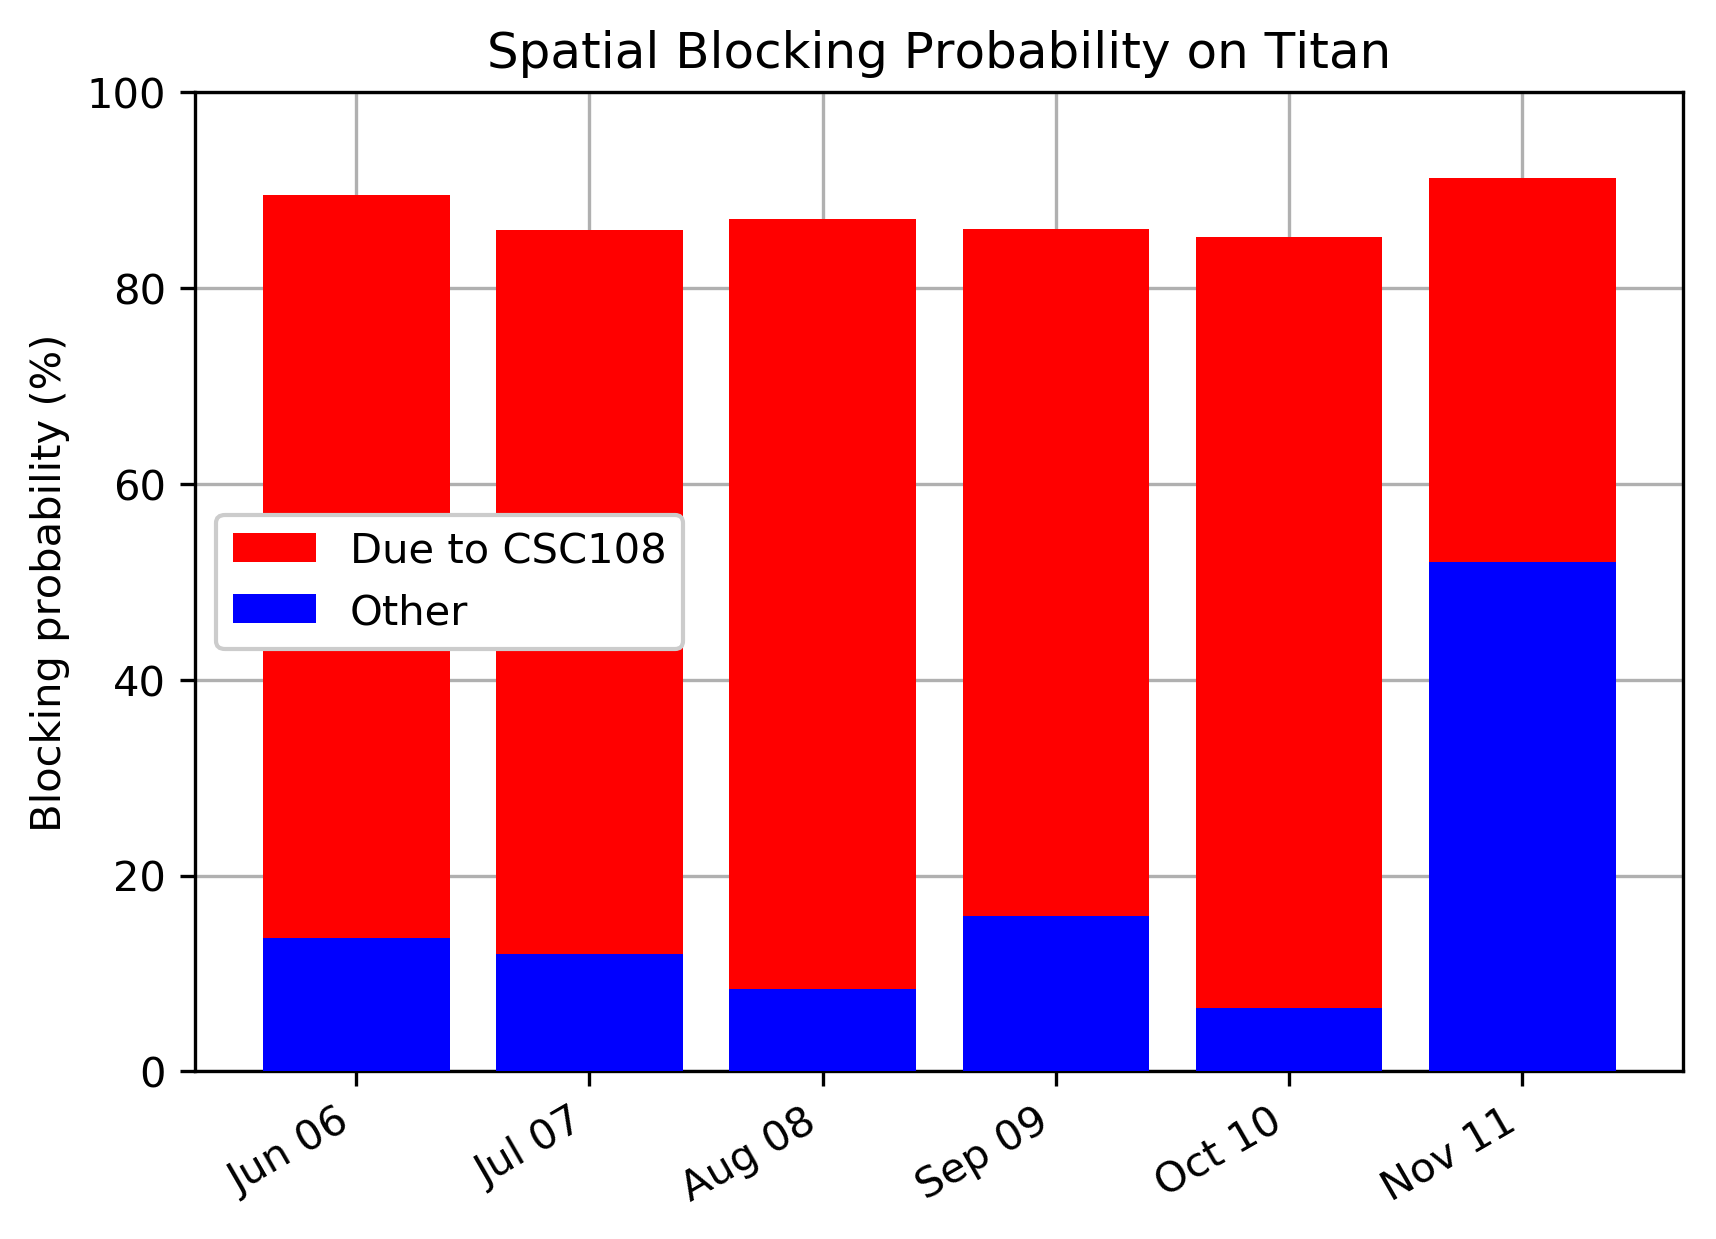
\includegraphics[width=0.4\textwidth]{images/barplot-spatial-blocking-by-month.png}}
  \subfloat[Temporal blocking\label{fig:temporal-blocking-by-month}]{
    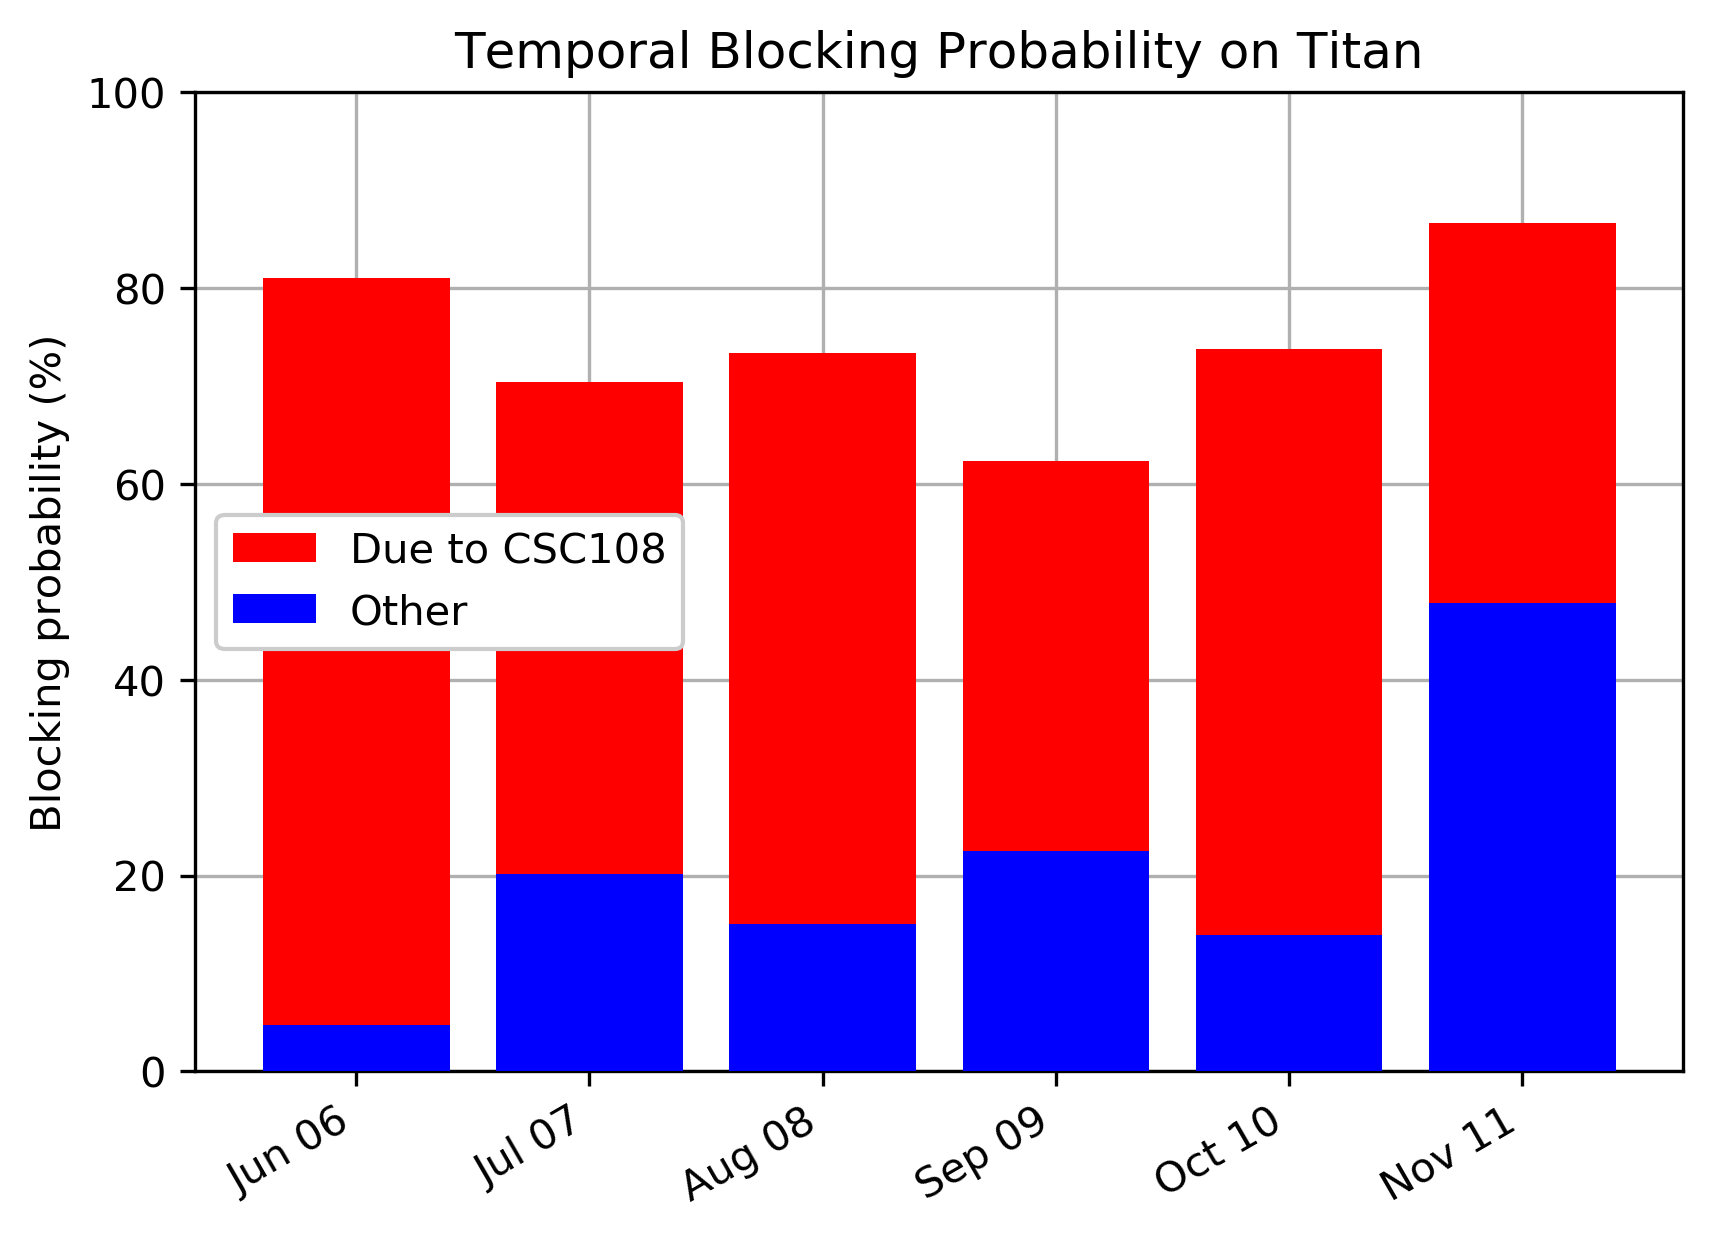
\includegraphics[width=0.4\textwidth]{images/barplot-temporal-blocking-by-month.png}}
  \caption{These plots depict the spatial and temporal blocking probabilities
by month for samples in which CSC108 was actively utilizing backfill
opportunity. The total height of the bars indicates the blocking probability
for the month, which is the proportion of samples in which at least one
eligible job was blocked. The red region indicates the percentage of samples in
which at least one eligible job would no longer be blocked if CSC108's jobs
were removed.}
\end{figure*}

% For two-column wide figures use
\begin{figure*}
% Use the relevant command to insert your figure file.
% For example, with the graphicx package use
  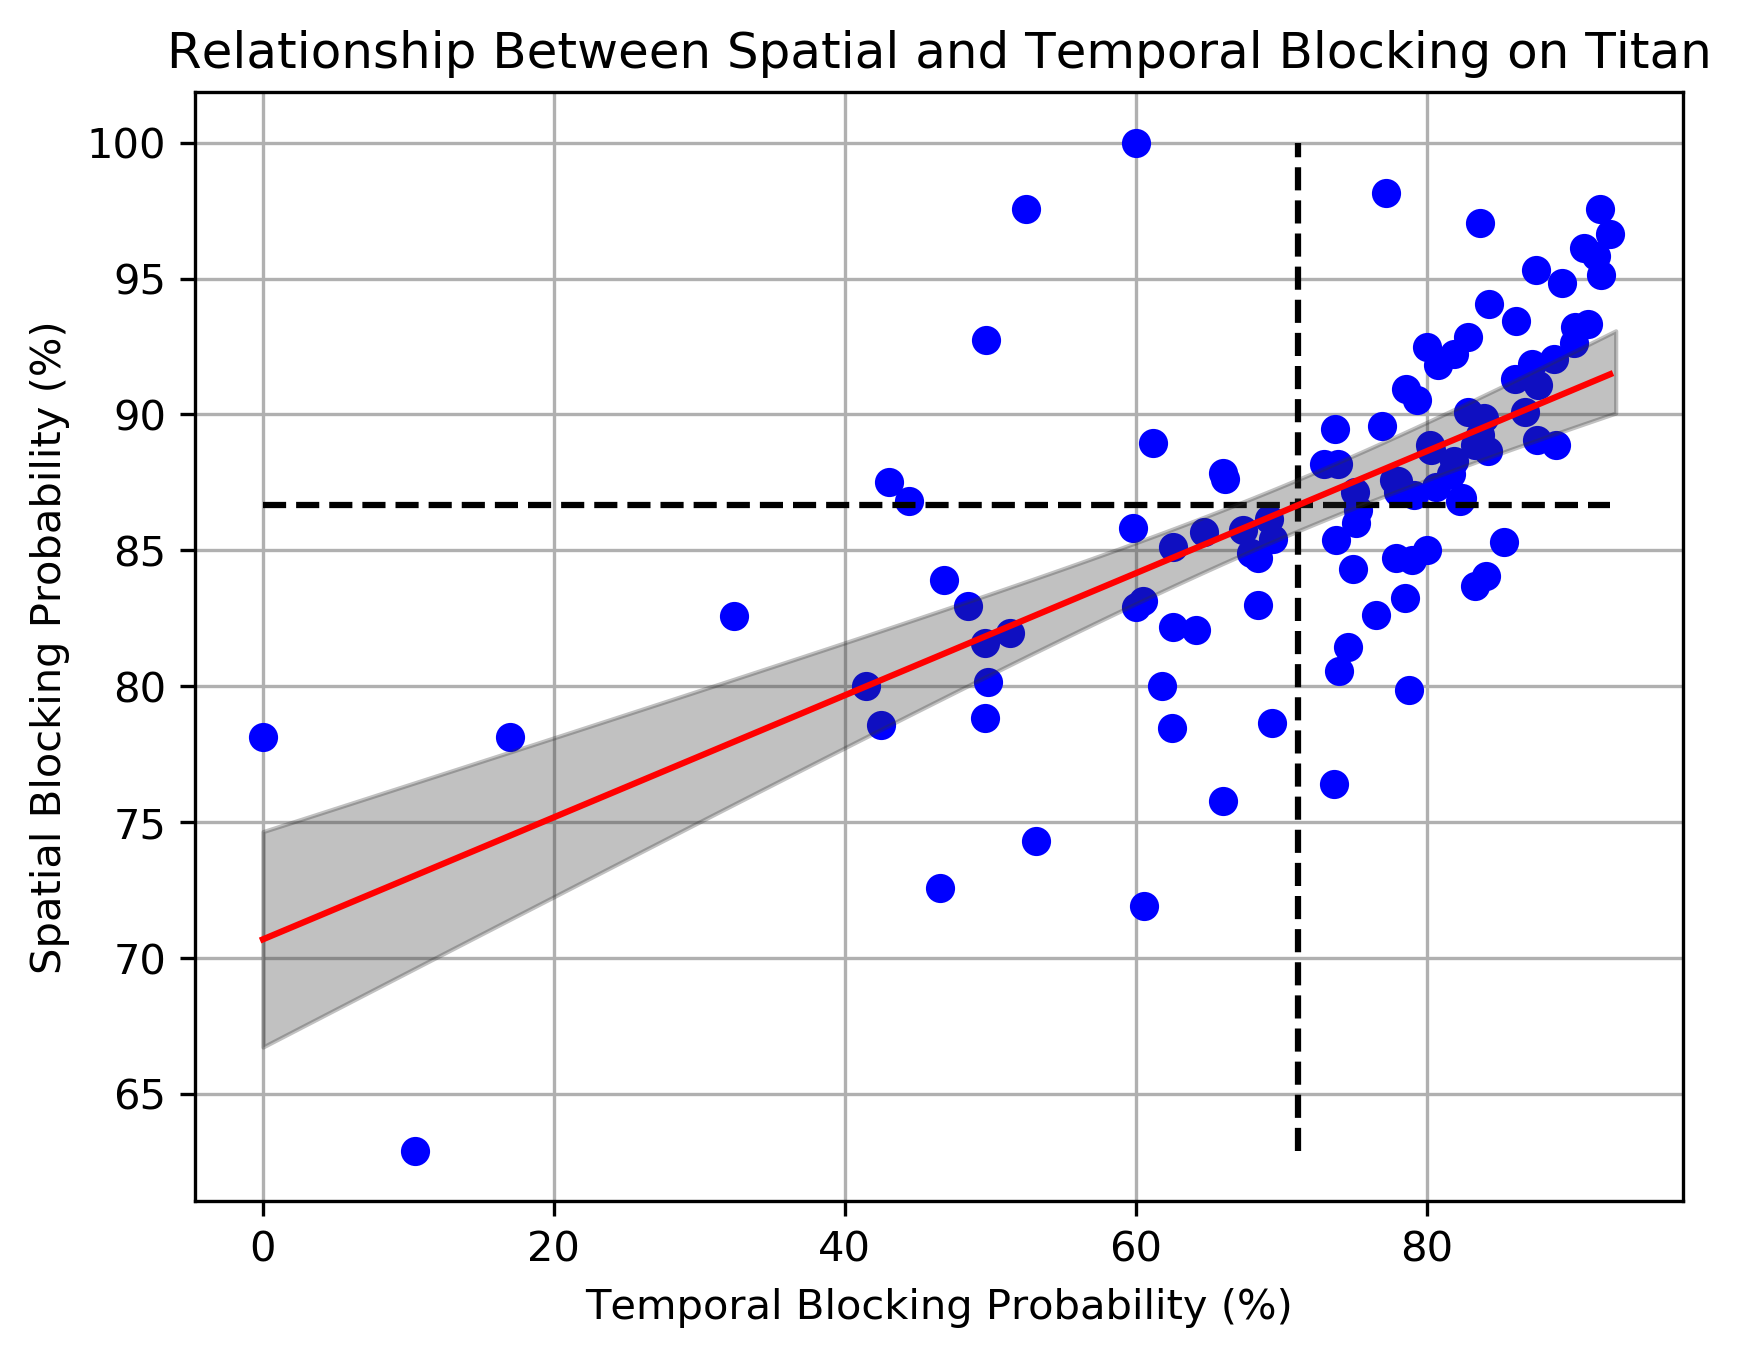
\includegraphics[width=0.75\textwidth]{images/linfit-spatial-vs-temporal-by-day.png}
% figure caption is below the figure
\caption{This figure demonstrates the relationship between spatial and temporal
blocking probabilities. Each blue point represents one day. The red line is an
Ordinary Least Squares (OLS) linear regression ($y = \beta_{1}x + \beta_0$)
with a slope $\beta_1$ of 0.2503 and an intercept $\beta_0$ of 68.7731. The
shaded gray areas represent 95\% confidence regions. The horizontal dotted
black line represents the mean spatial blocking probability for all points, and
the vertical dotted black line represents the mean temporal blocking
probability for all points. The $\text{R}^2$ value is 0.4410.}
\label{fig:spatial-vs-temporal}
\end{figure*}
%%%

Three indicators of system performance were chosen this time, as well, to
assess the impact of CSC108 on Titan: wait times, throughput, and utilization.
In order to map wait time to a value that can be attributed to a day, wait time
was defined in terms of an average wait time. Average wait time was defined as
the total number of hours spent waiting during a given day, per job that
appeared on that day. For example, a job which was submitted one day but which
did not run until the next day would contribute part of its wait time to the
first day and the rest to the second day, and it would be considered to have
appeared on both days. Throughput was defined as the number of jobs completed
per day, as before. Utilization was also defined as before, as the percentage
of core hours consumed out of the total core hours available.

%%% WAIT TIMES STUFF

Having established the two measures of blocking probability and their
relationship to one another, we followed the same techniques used in
Section~\ref{subsec:simple-linear-relationships} to create best-fit lines with
95\% confidence intervals, to investigate the relationships between blocking
probabilities and wait times experienced by jobs on Titan. Figures
\ref{fig:wait-time-spatial-all} and \ref{fig:wait-time-temporal-all} illustrate
the effects of spatial and temporal blocking probability on wait times, and
Figures \ref{fig:wait-time-spatial-csc108} and
\ref{fig:wait-time-temporal-csc108} show how CSC108's contribution to blocking
impacts wait times. More specifically, in Figures
\ref{fig:wait-time-spatial-csc108} and \ref{fig:wait-time-temporal-csc108}, the
values used for the blocking probabilities correspond to the red regions in
Figures \ref{fig:spatial-blocking-by-month} and
\ref{fig:temporal-blocking-by-month}, which indicate the percentage of samples
in which at least one eligible job would no longer be blocked if CSC108 freed
its resources. The qualitative interpretation for the wait time plots is that,
as competition for resources increases on Titan, average wait times decrease,
but when competition with CSC108 for nodes increases, average wait times
increase. Unfortunately, the goodness-of-fit values are again very poor.

\begin{figure*}
  \subfloat[Spatial blocking\label{fig:wait-time-spatial-all}]{
    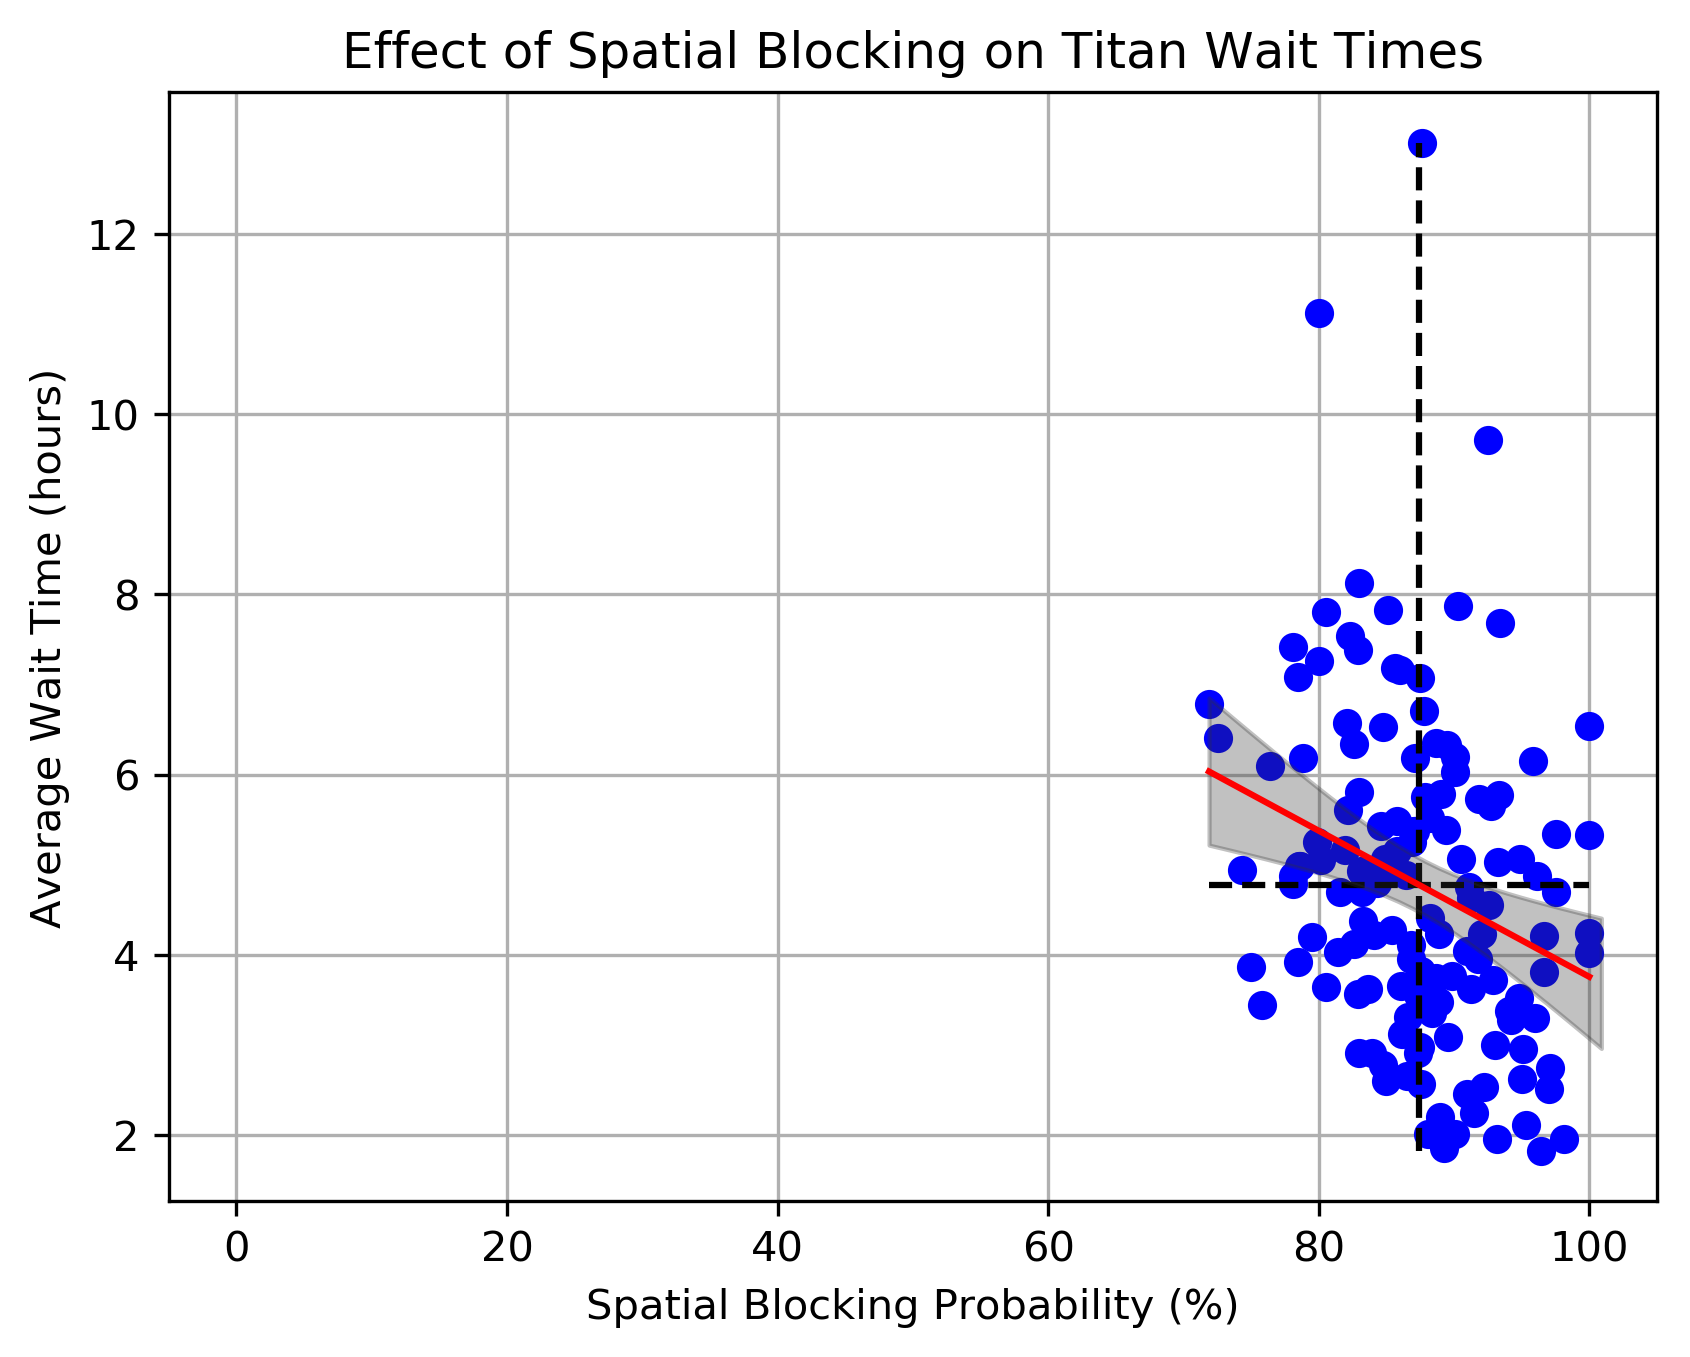
\includegraphics[width=0.4\textwidth]{images/linfit-wait-time-vs-spatial-blocking-by-day.png}}
  \subfloat[Temporal blocking\label{fig:wait-time-temporal-all}]{
    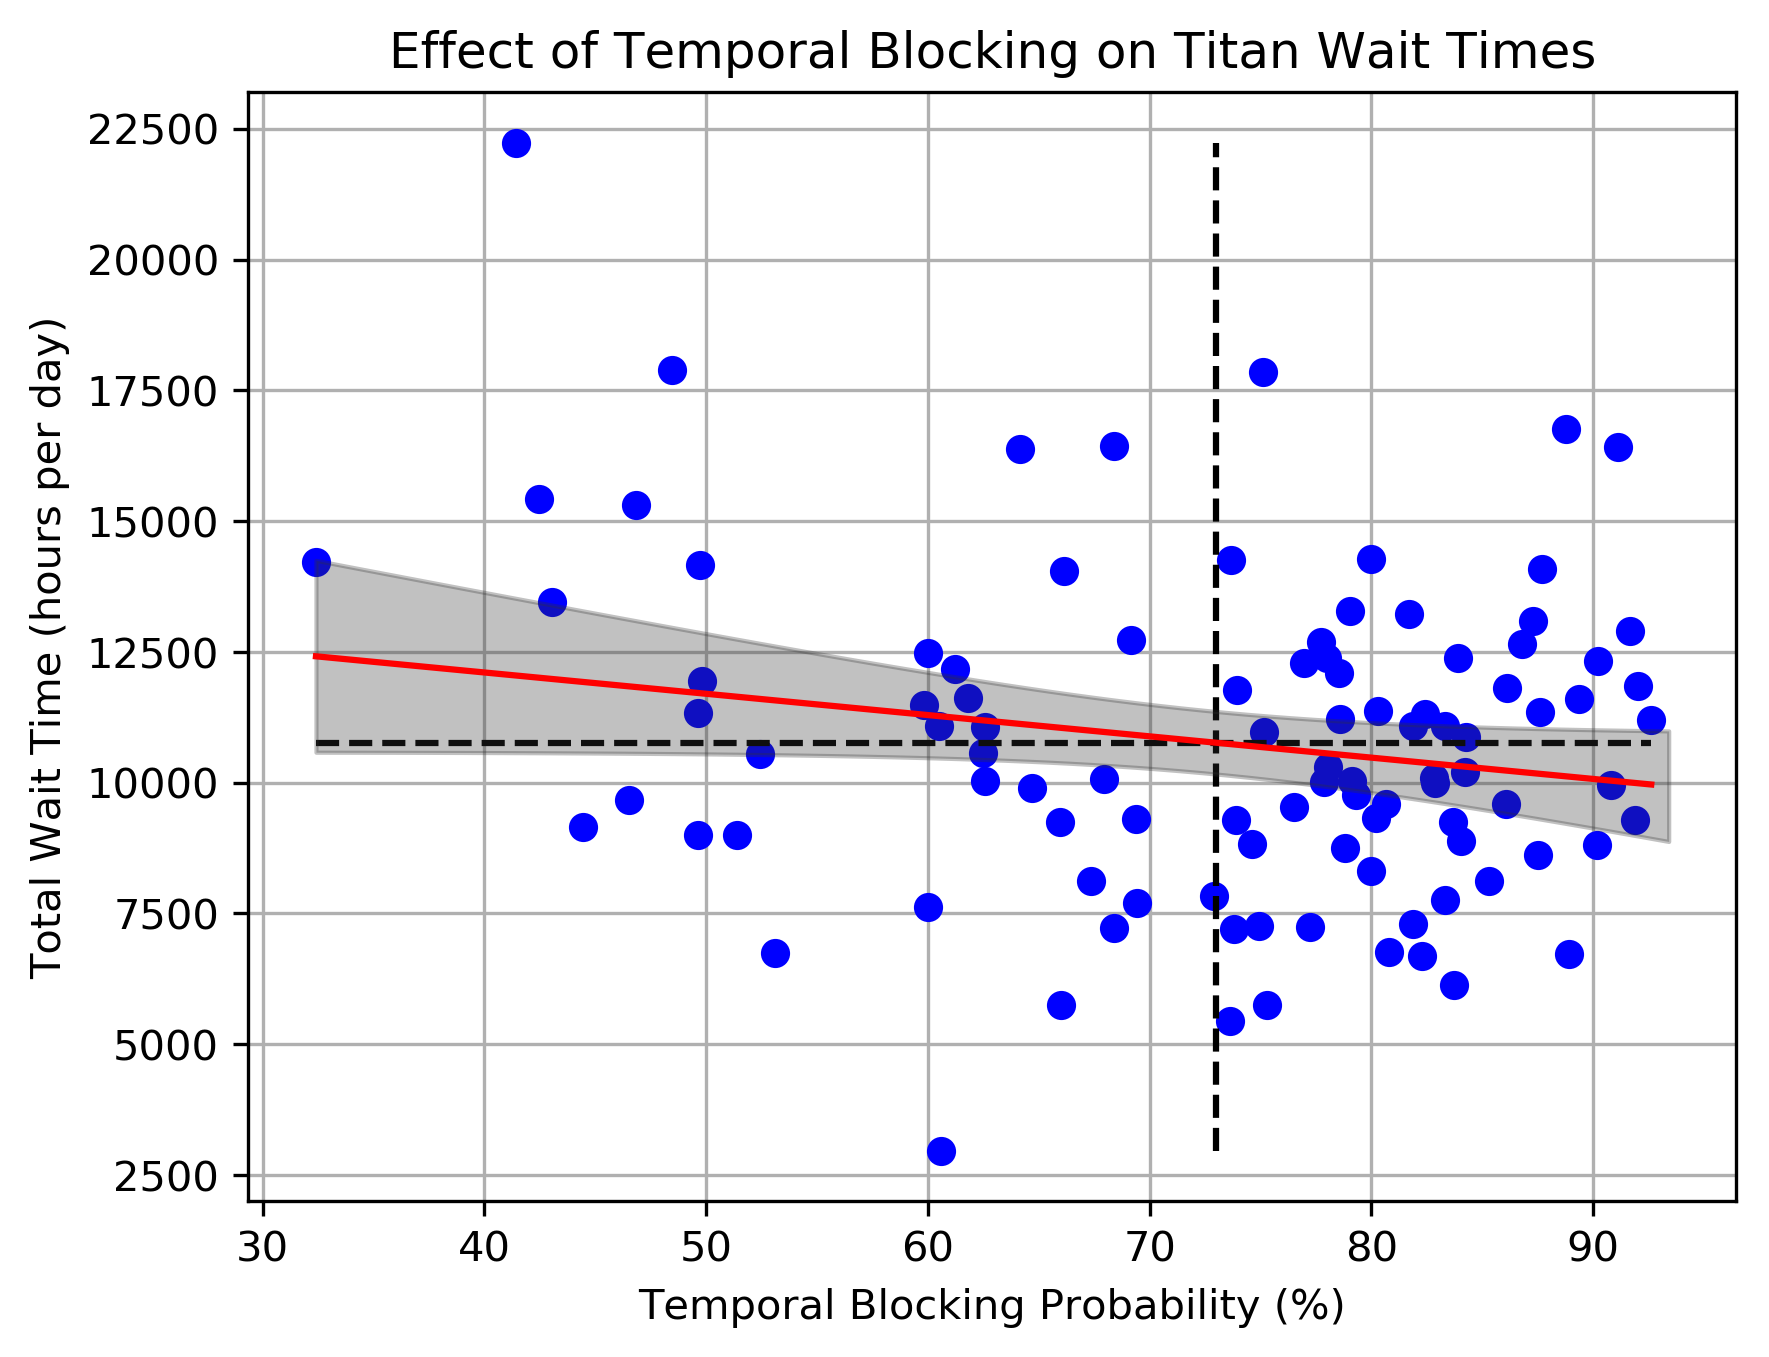
\includegraphics[width=0.4\textwidth]{images/linfit-wait-time-vs-temporal-blocking-by-day.png}}
  \vspace{1em}
  \subfloat[Spatial blocking by CSC108\label{fig:wait-time-spatial-csc108}]{
    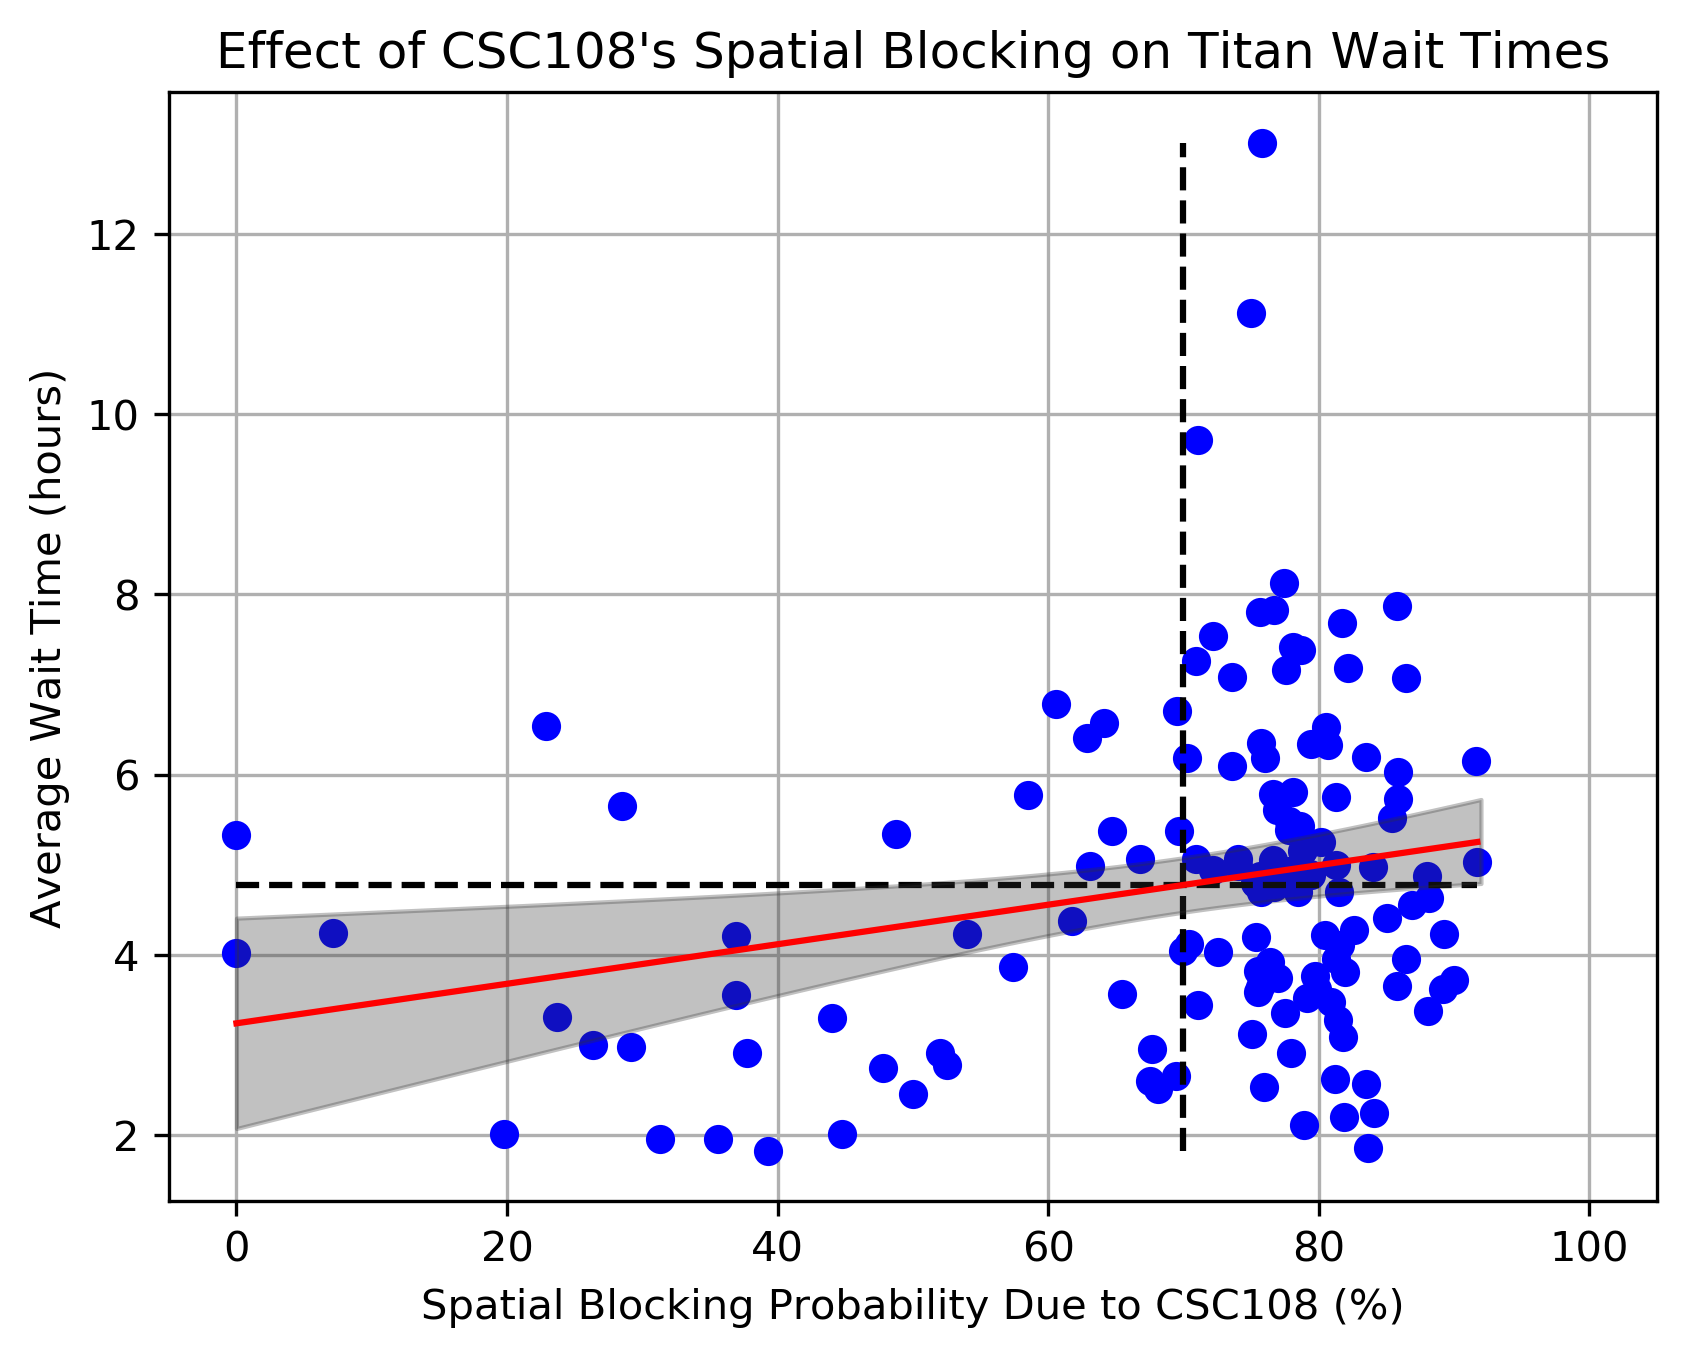
\includegraphics[width=0.4\textwidth]{images/linfit-wait-time-vs-csc108-spatial.png}}
  \subfloat[Temporal blocking by CSC108\label{fig:wait-time-temporal-csc108}]{
    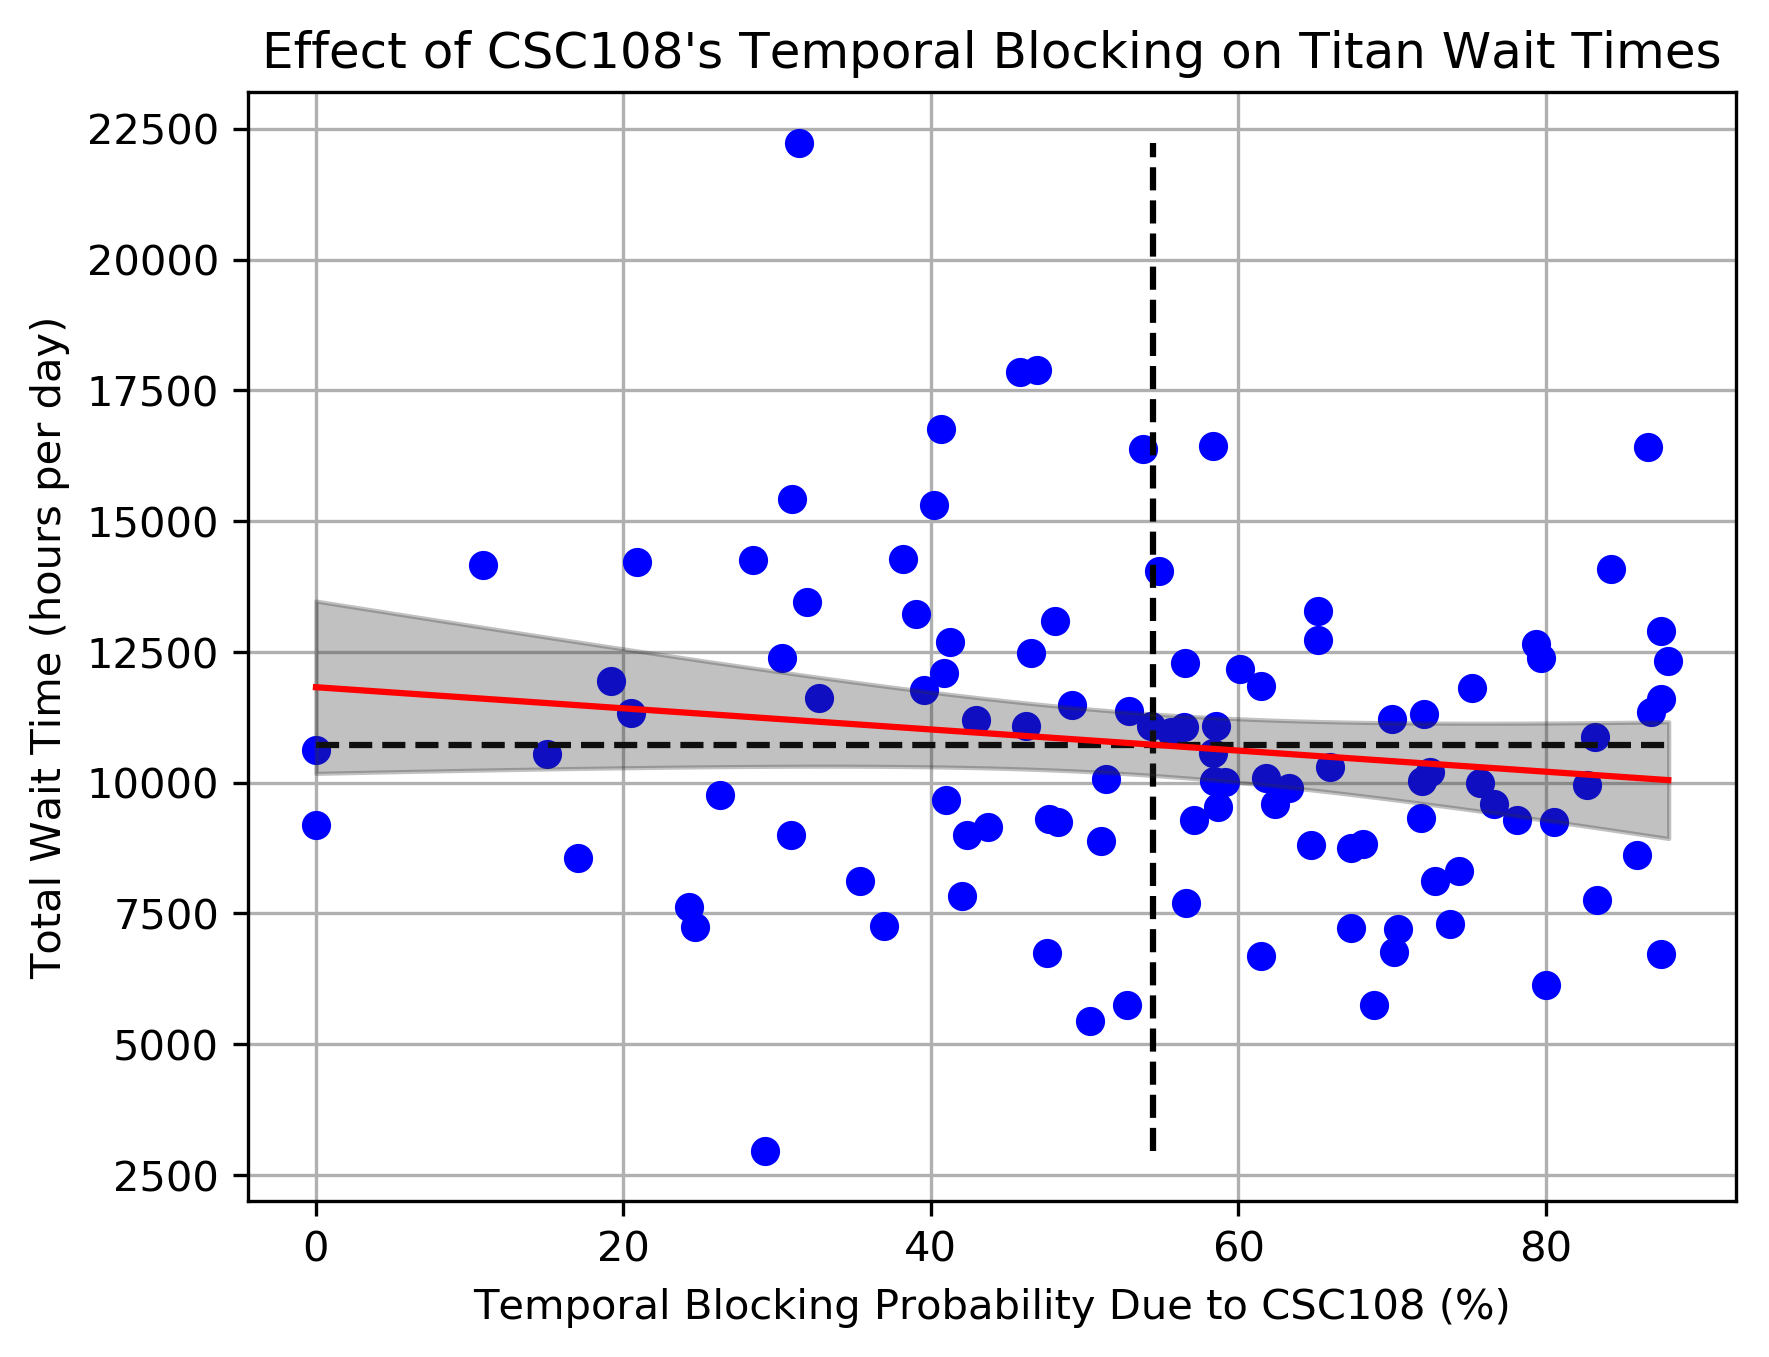
\includegraphics[width=0.4\textwidth]{images/linfit-wait-time-vs-csc108-temporal.png}}
  \caption{These plots demonstrate the relationships between the average wait
times on Titan and one-dimensional blocking probabilities. Each blue point
represents one day. Each red line is an Ordinary Least Squares (OLS) linear
regression with parameters given in Table~\ref{tab:blocking-wait-time-params}.
Each shaded gray area represents a 95\% confidence region. Each horizontal
dotted black line represents the mean wait times for all points in that plot,
and each vertical dotted black line represents the mean blocking probability
for all points in that plot.}
\end{figure*}

% For tables use
\begin{table}
% table caption is above the table
\caption{The table contains the parameter values for the Ordinary Least Squares
(OLS) linear regression models regarding blocking probabilities and average
wait times. The first column corresponds to the figure depicting the model,
while the second and third columns correspond the coefficients $\beta_1$ and
$\beta_0$ in the model $y = \beta_{1}x + \beta_0$.}
\label{tab:blocking-wait-time-params}       % Give a unique label
% For LaTeX tables use
\begin{tabular}{crrr}
\hline\noalign{\smallskip}
Figure  & Slope $\beta_1$ & Intercept $\beta_0$     & $\text{R}^2$ \\
\noalign{\smallskip}\hline\noalign{\smallskip}
\ref{fig:wait-time-spatial-all}     &   -0.0810 &   11.8610 &   0.0737  \\
\ref{fig:wait-time-temporal-all}    &   -0.0401 &    7.7491 &   0.1265  \\
\ref{fig:wait-time-spatial-csc108}  &    0.0219 &    3.2420 &   0.0509  \\
\ref{fig:wait-time-temporal-csc108} &   -0.0102 &    5.3217 &   0.0147  \\
\noalign{\smallskip}\hline
\end{tabular}
\end{table}

%%% THROUGHPUT STUFF

Figures \ref{fig:throughput-spatial-all}, \ref{fig:throughput-temporal-all},
\ref{fig:throughput-spatial-csc108}, and \ref{fig:throughput-temporal-csc108}
are all in agreement that increasing competition corresponds to increasing
throughput, in units of jobs completed per day. The goodness-of-fit values are
poor, however, as shown in Table~\ref{tab:blocking-throughput-params}, so these qualitative results may only be said to be suggestive.

%%%
\begin{figure*}
  \subfloat[Spatial blocking\label{fig:throughput-spatial-all}]{
    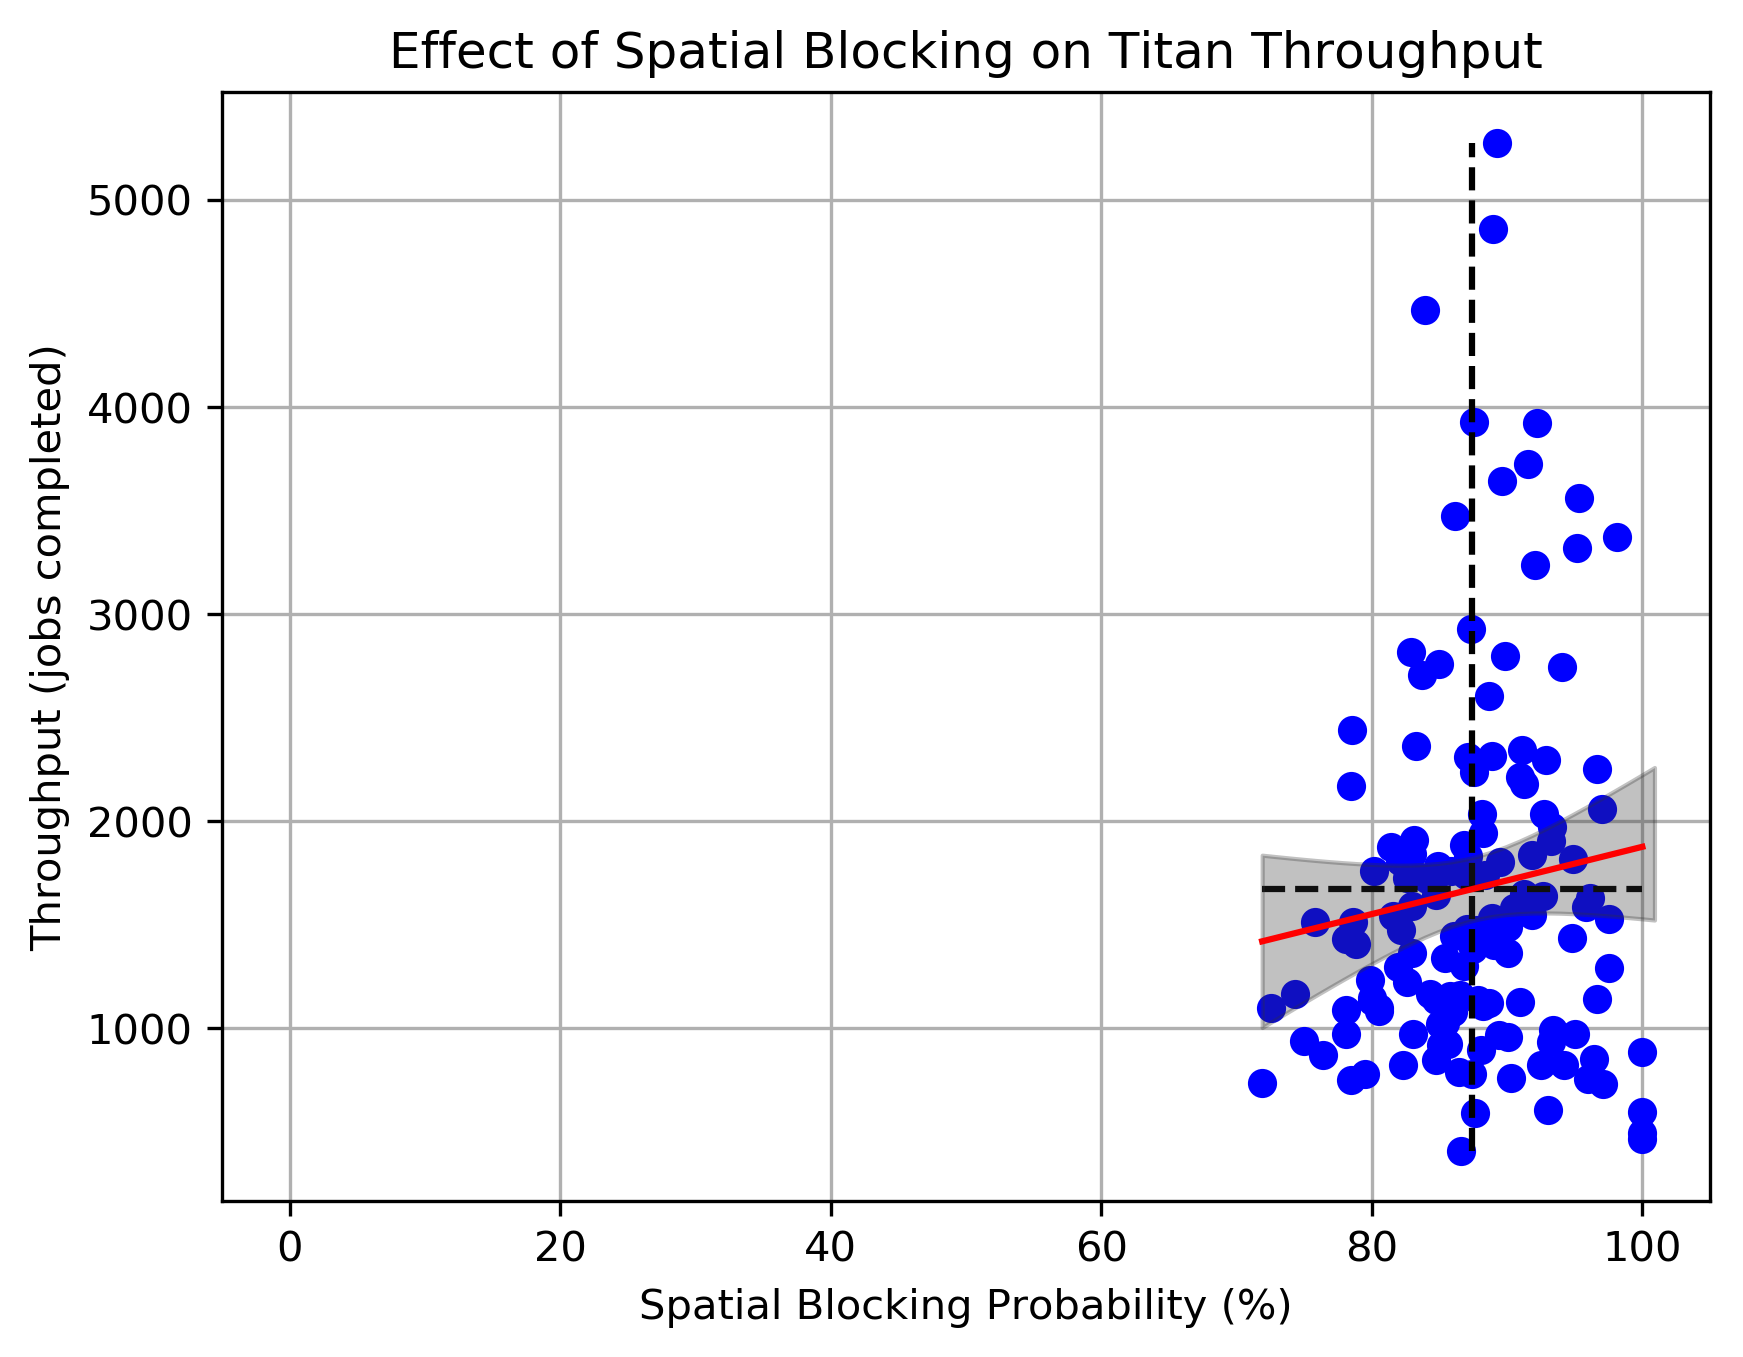
\includegraphics[width=0.4\textwidth]{images/linfit-throughput-vs-spatial-blocking.png}}
  \subfloat[Temporal blocking\label{fig:throughput-temporal-all}]{
    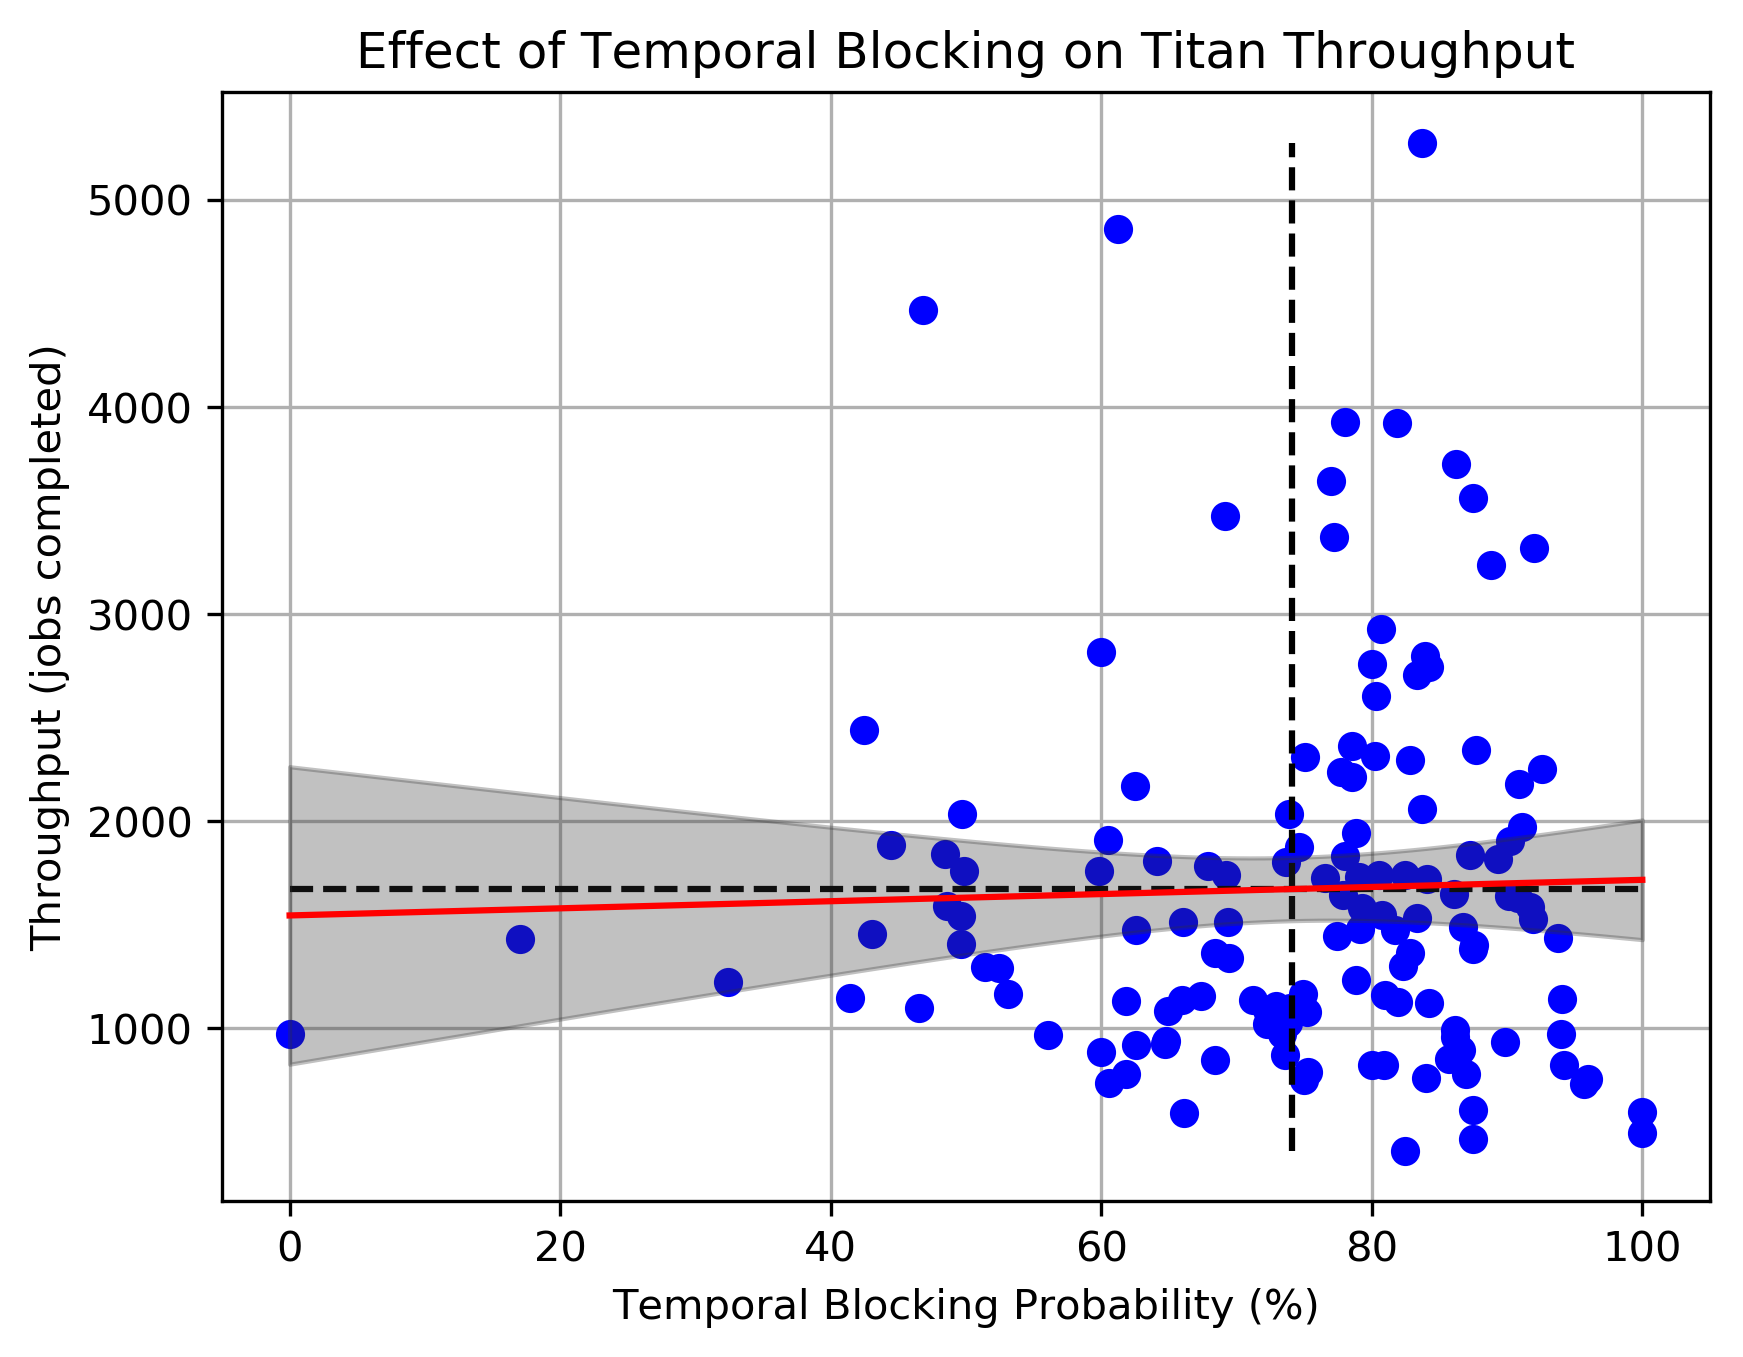
\includegraphics[width=0.4\textwidth]{images/linfit-throughput-vs-temporal-blocking.png}}
  \vspace{1em}
  \subfloat[Spatial blocking by CSC108\label{fig:throughput-spatial-csc108}]{
    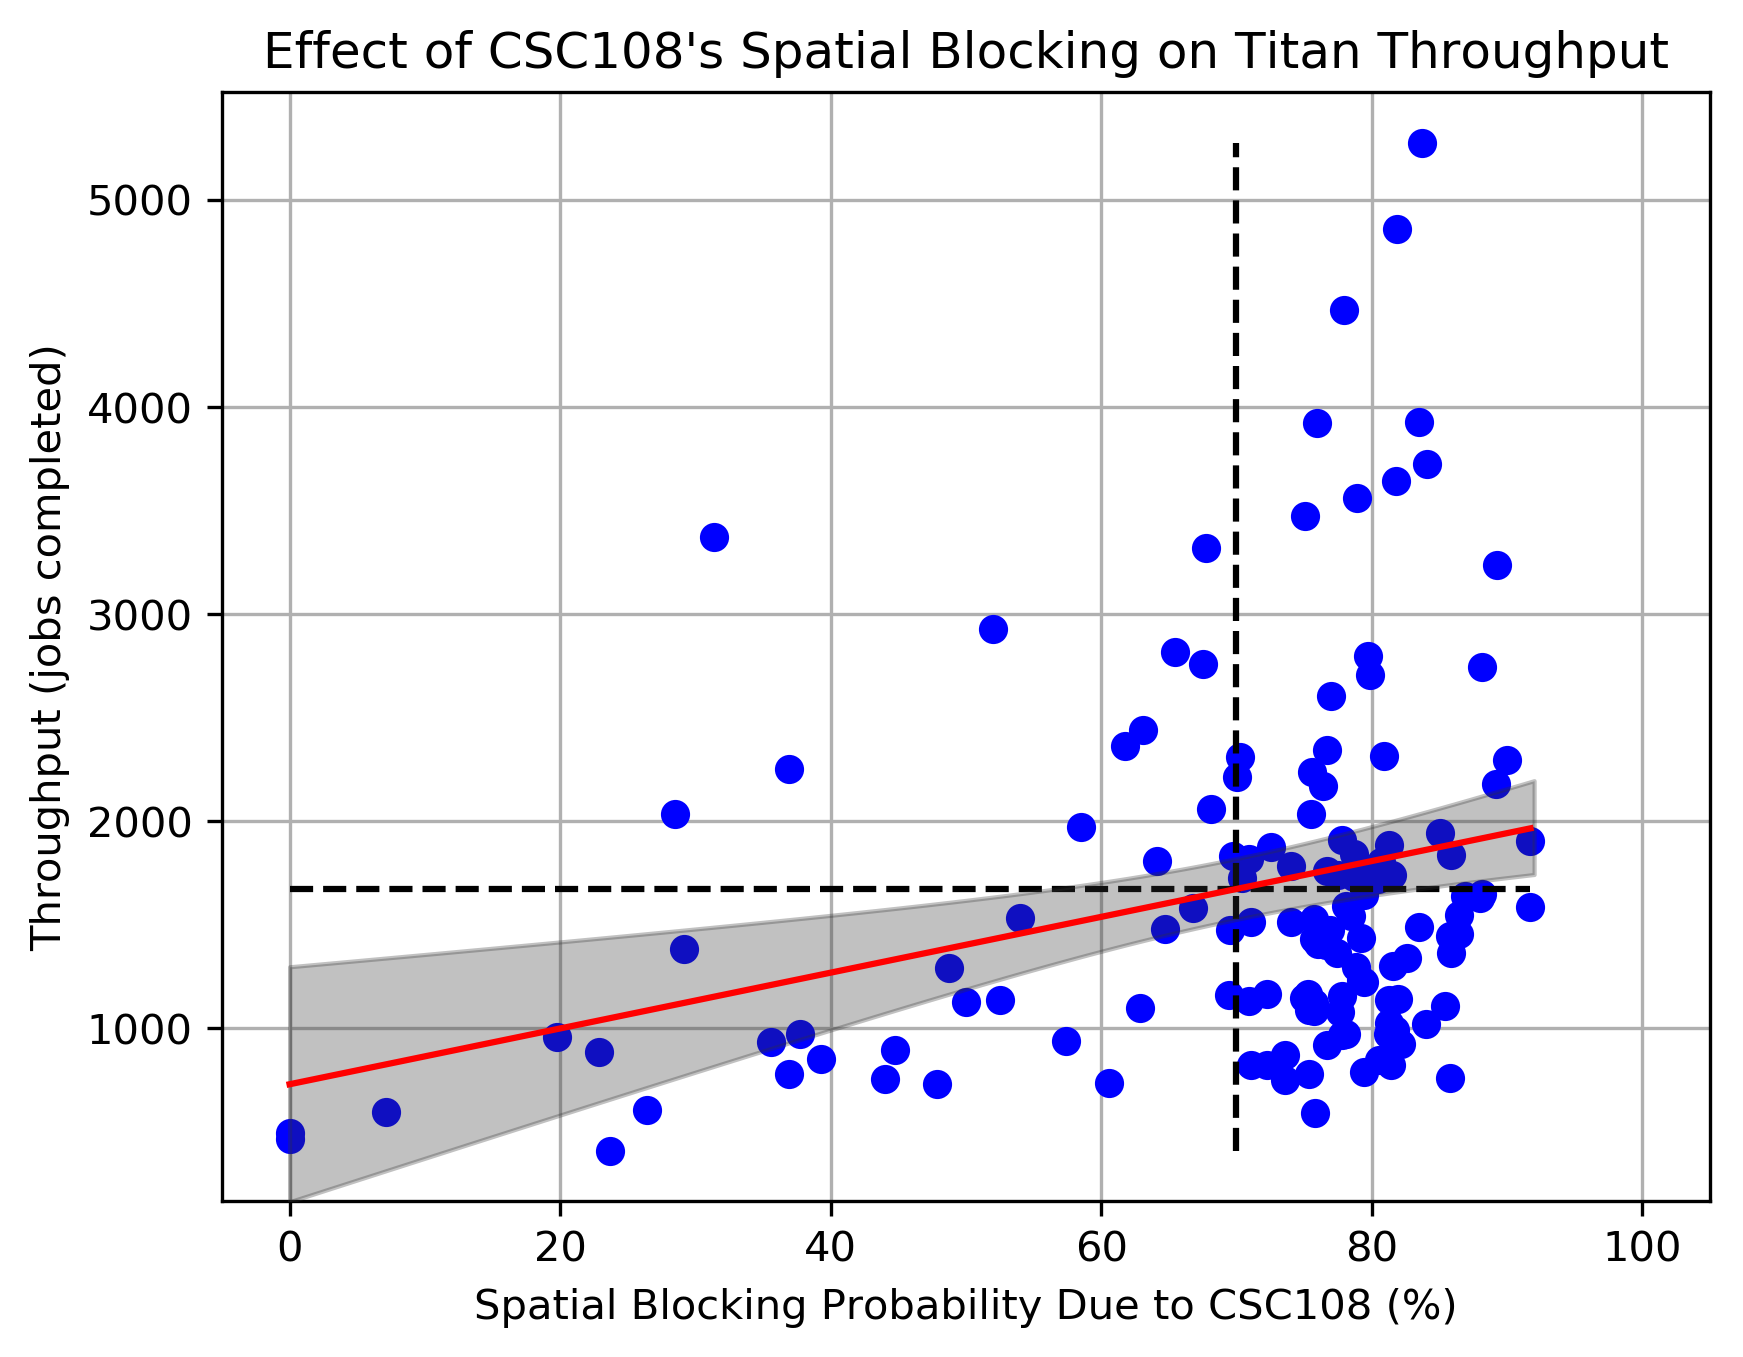
\includegraphics[width=0.4\textwidth]{images/linfit-throughput-vs-csc108-spatial.png}}
  \subfloat[Temporal blocking by CSC108\label{fig:throughput-temporal-csc108}]{
    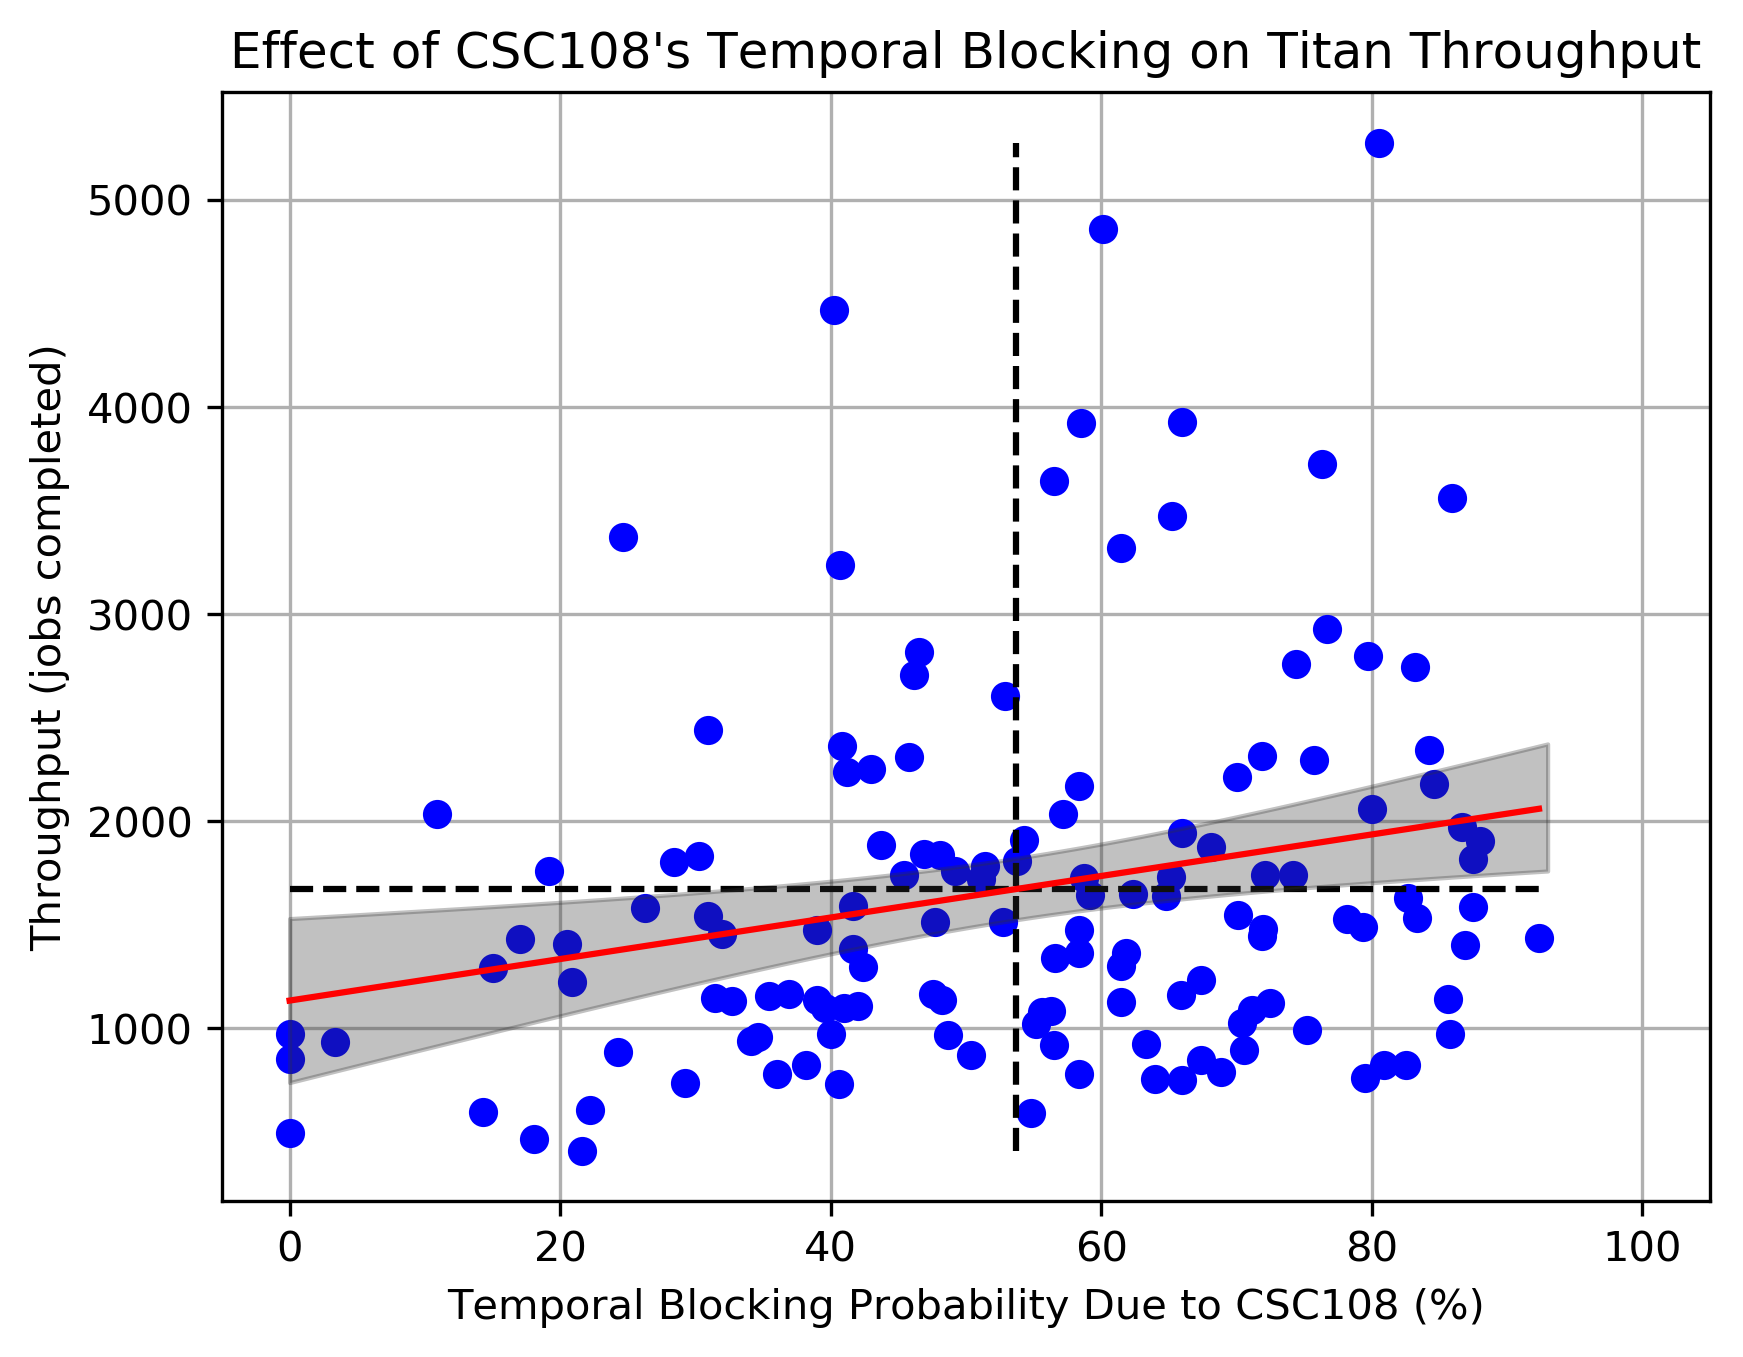
\includegraphics[width=0.4\textwidth]{images/linfit-throughput-vs-csc108-temporal.png}}
  \caption{These plots demonstrate the relationships between throughput on
Titan and one-dimensional blocking probabilities. Each blue point represents
one day. Each red line is an Ordinary Least Squares (OLS) linear regression
with parameters given in Table~\ref{tab:blocking-throughput-params}. Each
shaded gray area represents a 95\% confidence region. Each horizontal dotted
black line represents the mean wait times for all points in that plot, and each
vertical dotted black line represents the mean blocking probability for all
points in that plot.}
\end{figure*}

% For tables use
\begin{table}
% table caption is above the table
\caption{The table contains the parameter values for the Ordinary Least Squares
(OLS) linear regression models regarding blocking probabilities and throughput.
The first column corresponds to the figure depicting the model, while the
second and third columns correspond the coefficients $\beta_1$ and $\beta_0$ in
the model $y = \beta_{1}x + \beta_0$.}
\label{tab:blocking-throughput-params}       % Give a unique label
% For LaTeX tables use
\begin{tabular}{crrr}
\hline\noalign{\smallskip}
Figure  & Slope $\beta_1$ & Intercept $\beta_0$     & $\text{R}^2$ \\
\noalign{\smallskip}\hline\noalign{\smallskip}
\ref{fig:throughput-spatial-all}     &  16.2402 &   252.3652    &   0.0122  \\
\ref{fig:throughput-temporal-all}    &   1.7196 &  1544.9669    &   0.0010  \\
\ref{fig:throughput-spatial-csc108}  &  13.4683 &   730.0687    &   0.0790  \\
\ref{fig:throughput-temporal-csc108} &  10.0245 &  1134.0212    &   0.0587  \\
\noalign{\smallskip}\hline
\end{tabular}
\end{table}
%%%

%%% UTILIZATION STUFF

Finally, we searched for simple linear relationships between the different
blocking probabilities and overall utilization on Titan. Figures
\ref{fig:utilization-spatial-all}, \ref{fig:utilization-temporal-all},
\ref{fig:utilization-spatial-csc108}, and \ref{fig:utilization-temporal-csc108}
do not ``agree'' like the throughput plots did, but three plots suggest an
interpretation in which increasing competition, indicated by increasing
blocking probability, corresponds to decreased utilization. The fourth plot,
which indicates competition with CSC108, relates increased competition to
increased utilization. Once again, the goodness-of-fit values are poor, as
shown in Table~\ref{tab:blocking-utilization-params}.

%%%
\begin{figure*}
  \subfloat[Spatial blocking\label{fig:utilization-spatial-all}]{
    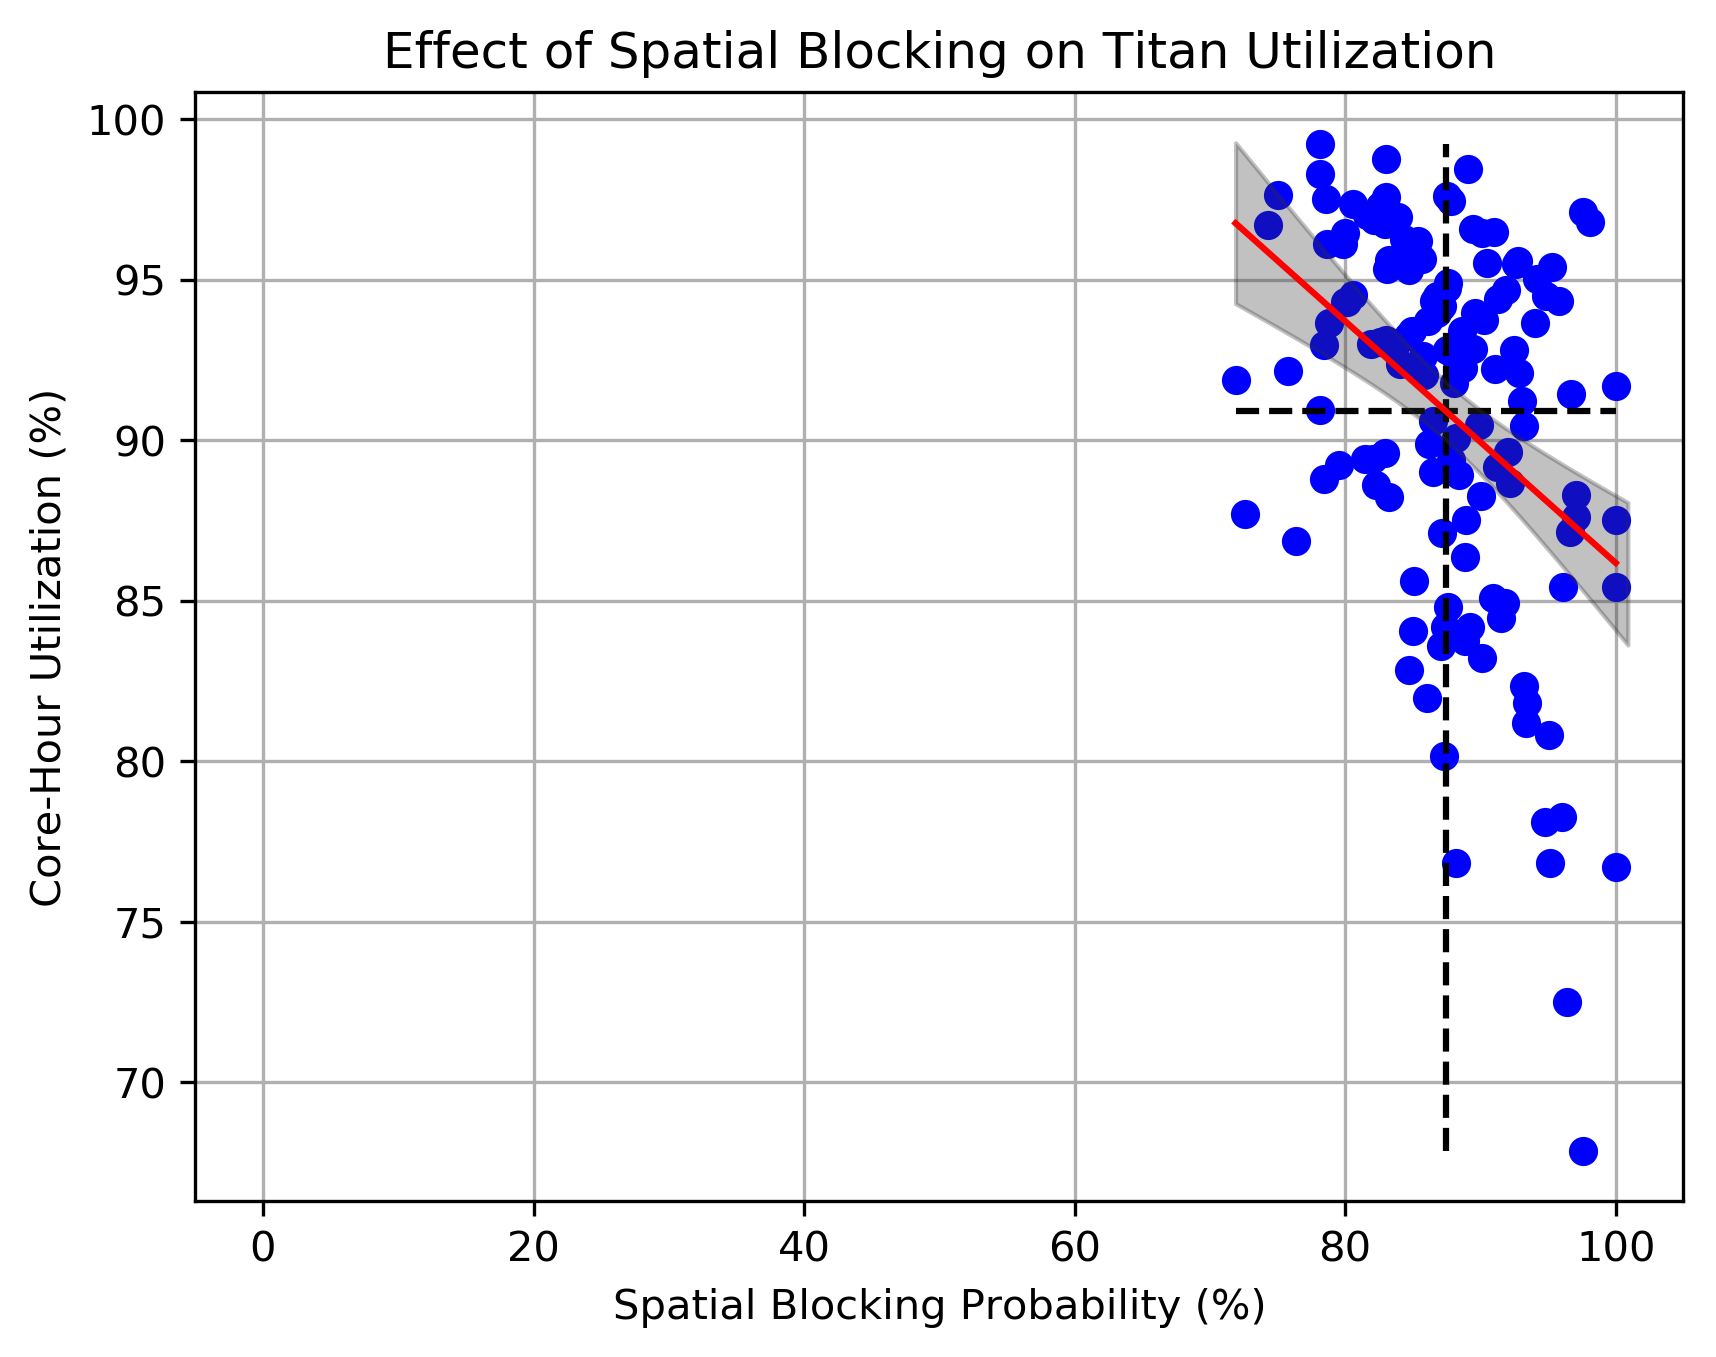
\includegraphics[width=0.4\textwidth]{images/linfit-utilization-vs-spatial-blocking.png}}
  \subfloat[Temporal blocking\label{fig:utilization-temporal-all}]{
    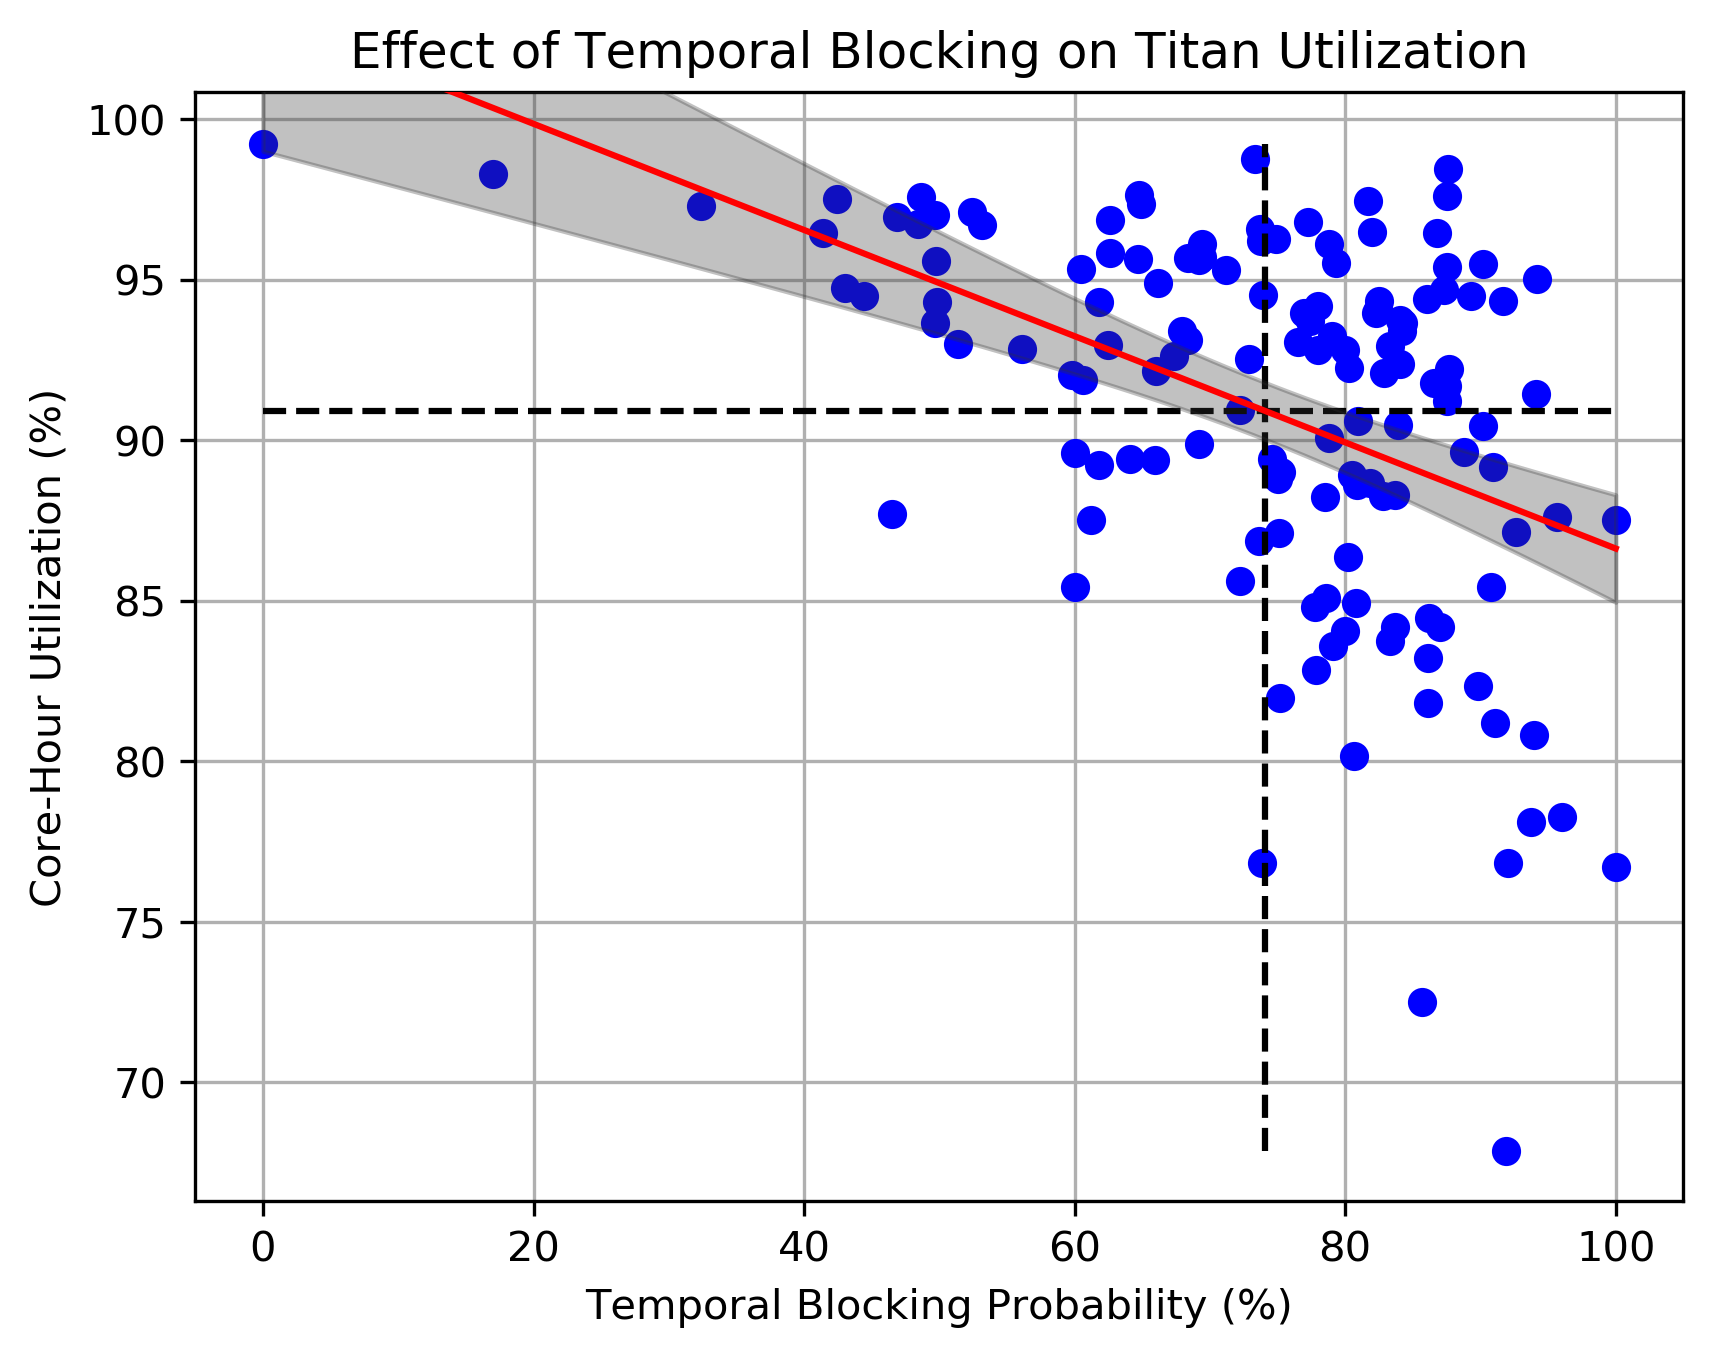
\includegraphics[width=0.4\textwidth]{images/linfit-utilization-vs-temporal-blocking.png}}
  \vspace{1em}
  \subfloat[Spatial blocking by CSC108\label{fig:utilization-spatial-csc108}]{
    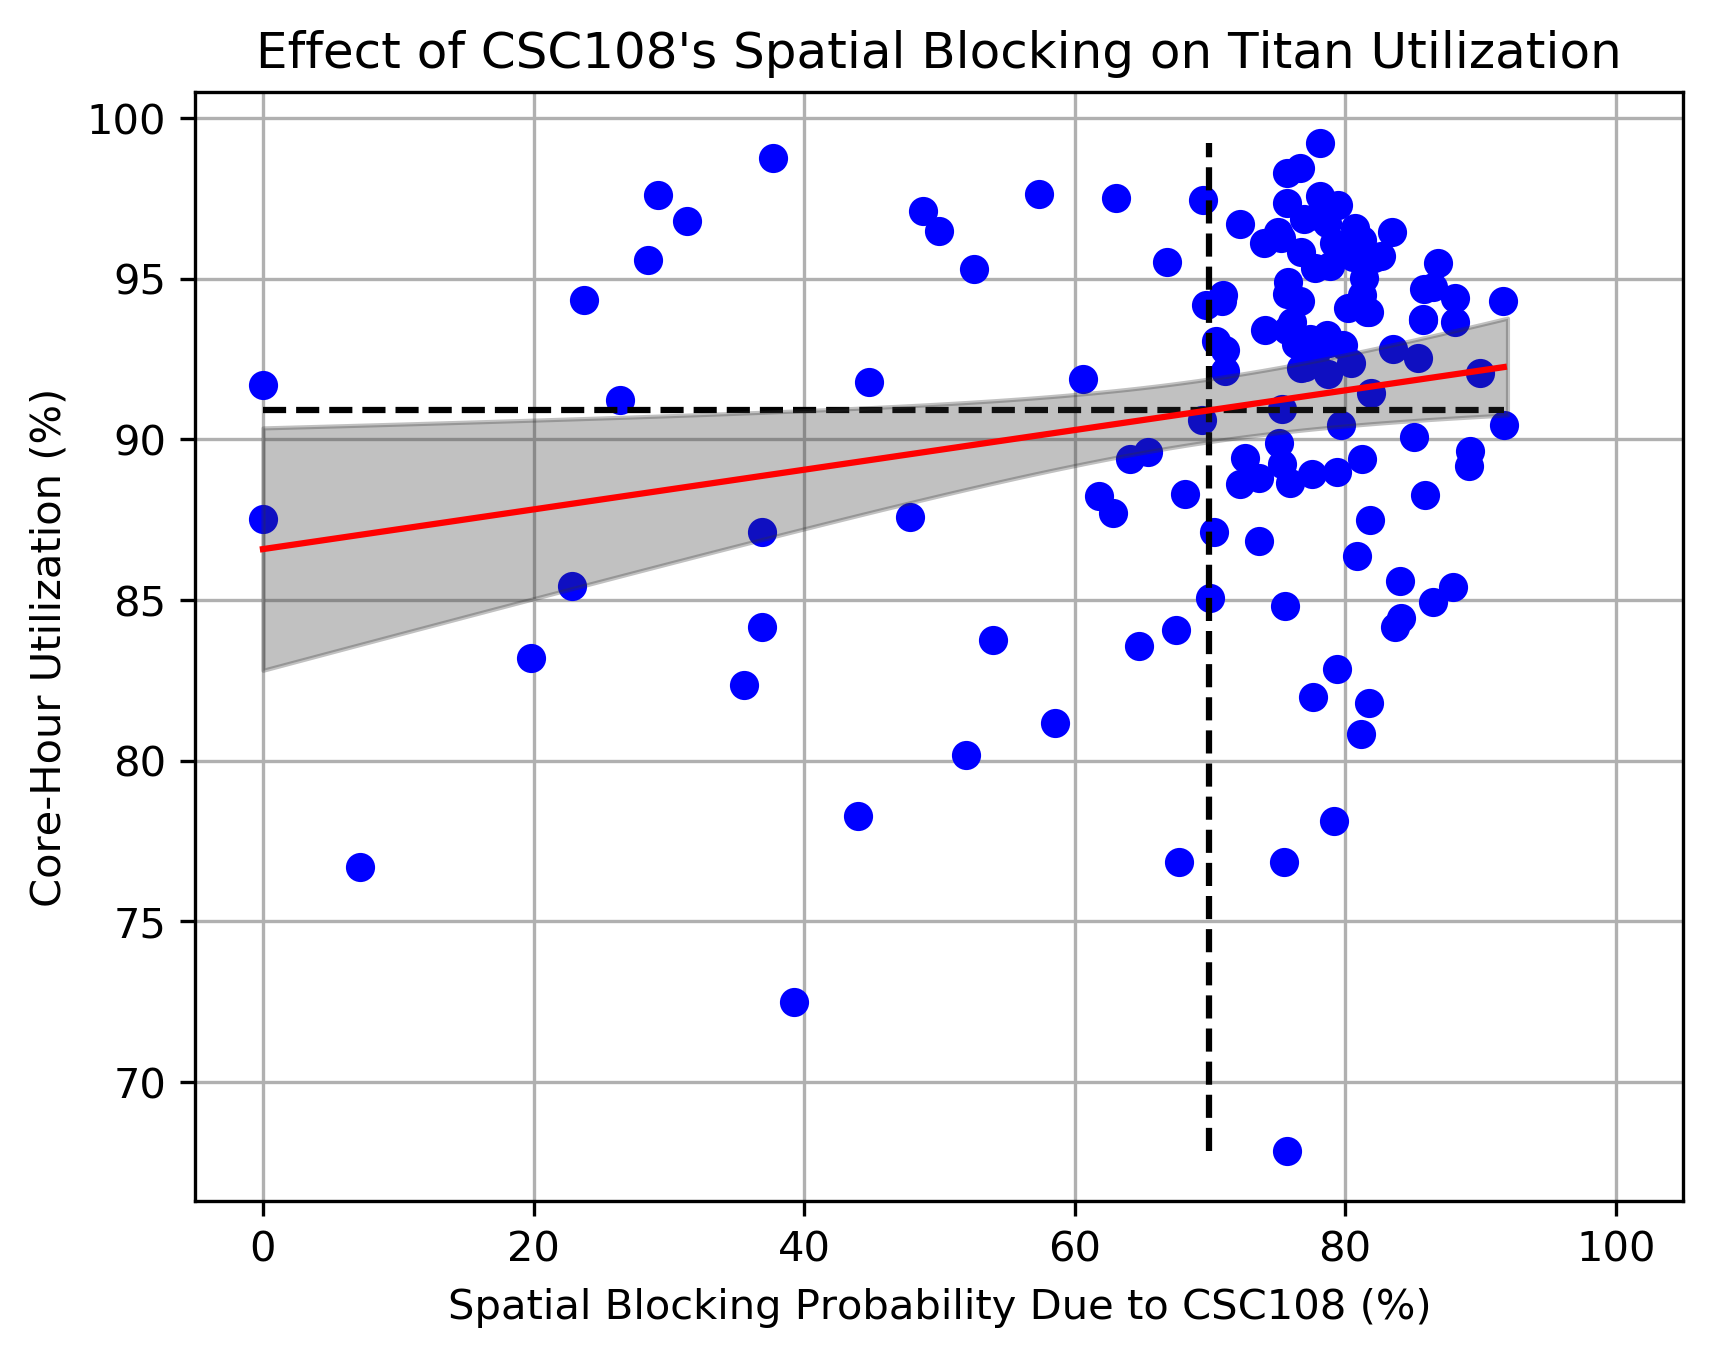
\includegraphics[width=0.4\textwidth]{images/linfit-utilization-vs-csc108-spatial.png}}
  \subfloat[Temporal blocking by CSC108\label{fig:utilization-temporal-csc108}]{
    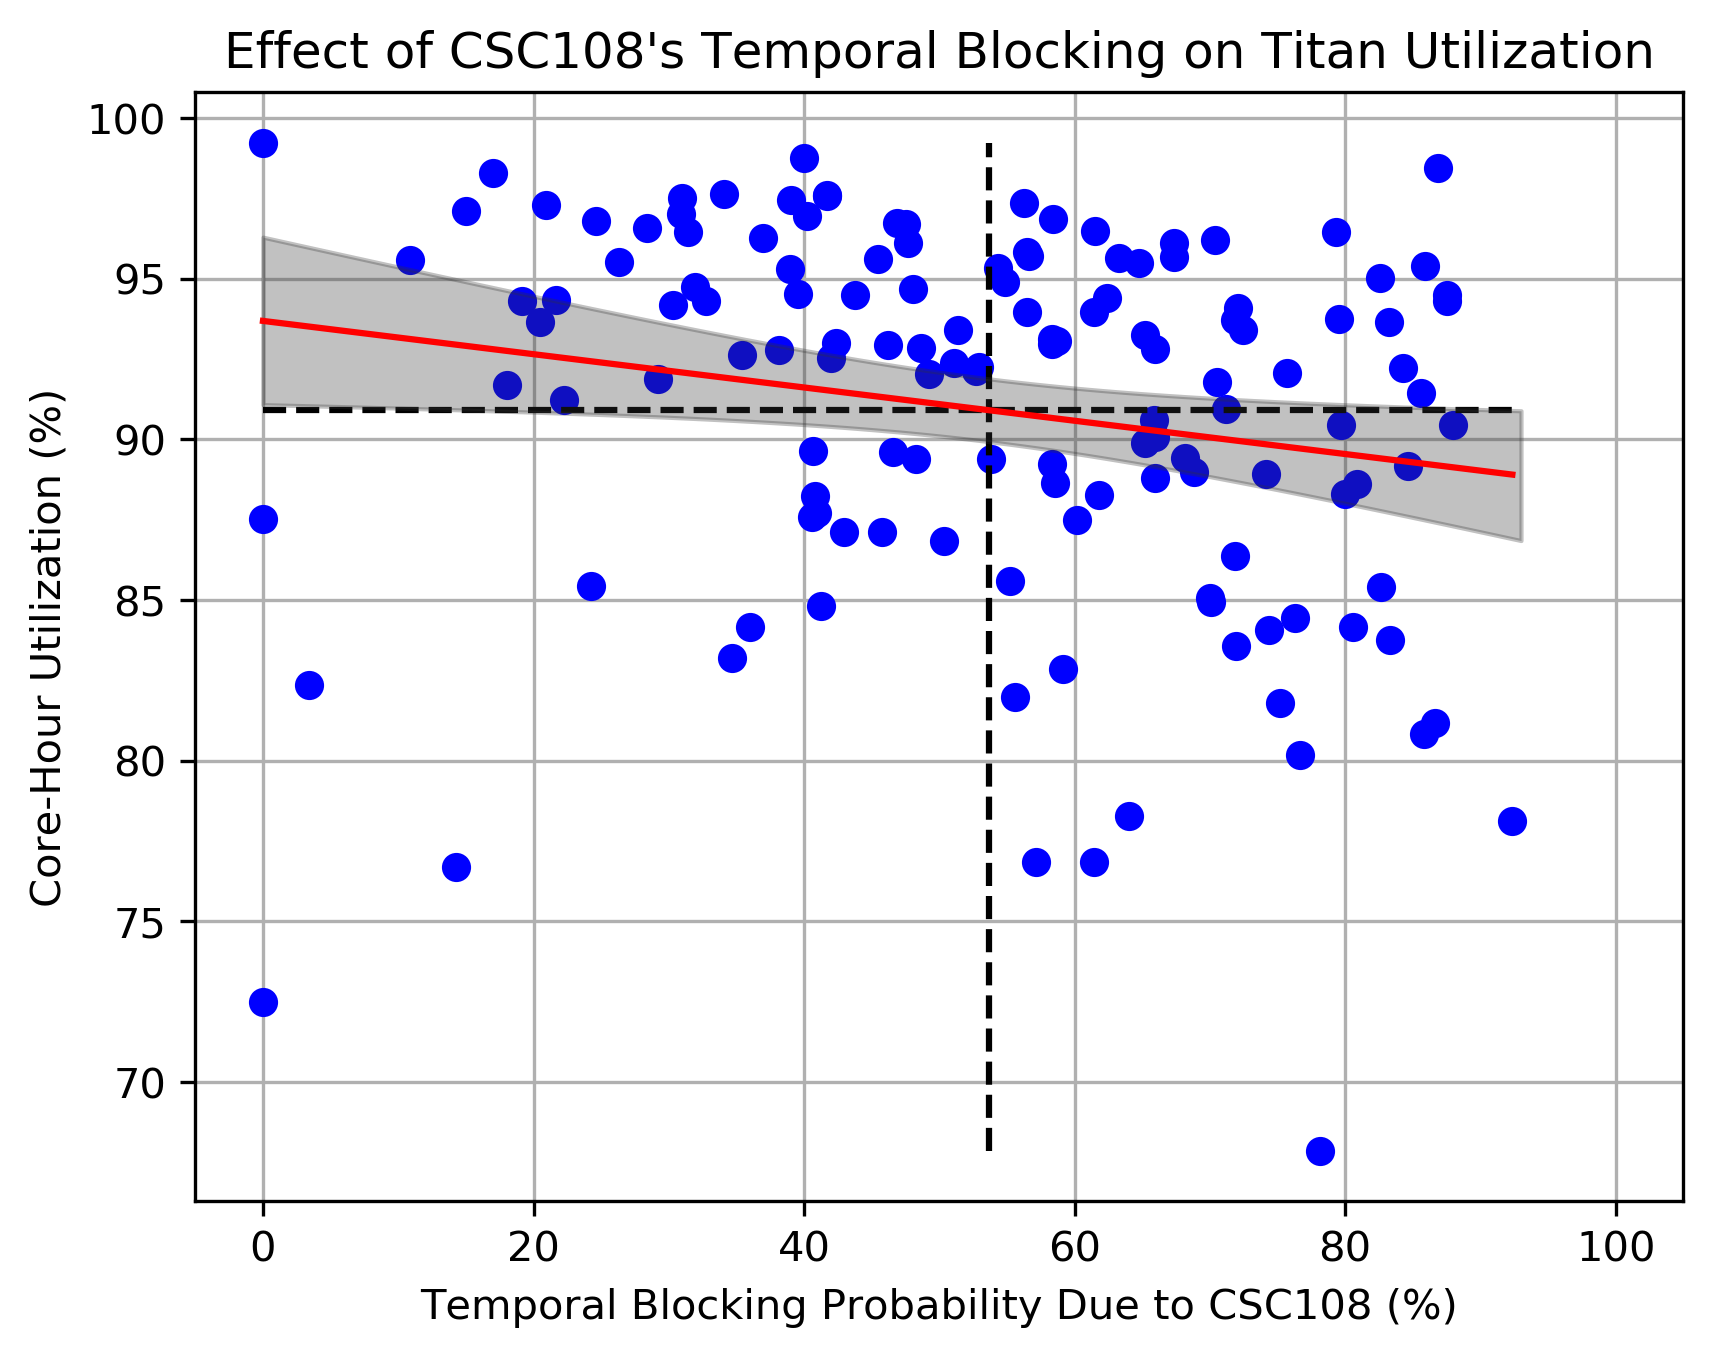
\includegraphics[width=0.4\textwidth]{images/linfit-utilization-vs-csc108-temporal.png}}
  \caption{These plots demonstrate the relationships between utilization on
Titan and one-dimensional blocking probabilities. Each blue point represents
one day. Each red line is an Ordinary Least Squares (OLS) linear regression
with parameters given in Table~\ref{tab:blocking-utilization-params}. Each
shaded gray area represents a 95\% confidence region. Each horizontal dotted
black line represents the mean wait times for all points in that plot, and each
vertical dotted black line represents the mean blocking probability for all
points in that plot.}
\end{figure*}

% For tables use
\begin{table}
% table caption is above the table
\caption{The table contains the parameter values for the Ordinary Least Squares
(OLS) linear regression models regarding blocking probabilities and utilization.
The first column corresponds to the figure depicting the model, while the
second and third columns correspond the coefficients $\beta_1$ and $\beta_0$ in
the model $y = \beta_{1}x + \beta_0$.}
\label{tab:blocking-utilization-params}       % Give a unique label
% For LaTeX tables use
\begin{tabular}{crrr}
\hline\noalign{\smallskip}
Figure  & Slope $\beta_1$ & Intercept $\beta_0$     & $\text{R}^2$ \\
\noalign{\smallskip}\hline\noalign{\smallskip}
\ref{fig:utilization-spatial-all}       &   -0.3766 &   123.8332 & 0.1543 \\
\ref{fig:utilization-temporal-all}    &     -0.1654 &   103.1603 & 0.2084 \\
\ref{fig:utilization-spatial-csc108}  &      0.0617 &    86.5830 & 0.0391 \\
\ref{fig:utilization-temporal-csc108} &     -0.0518 &    93.6845 & 0.0370 \\
\noalign{\smallskip}\hline
\end{tabular}
\end{table}
%%%

Thus, the use of blocking probability provided additional insight regarding the
impact of CSC108 on Titan, but just like in
Section~\ref{subsec:simple-linear-relationships}, the best-fit lines all
displayed very poor goodness-of-fit, rendering the interpretations somewhat
weak.

%%%%%%%%%%%%%%%%%%%%%%%%%%%%%%%%%%%%%%%%%%%%%%%%%%%%%%%%%%%%%%%%%%%%%%%%%%%%%%%%
\subsection{Summary}
\label{subsec:performance-summary}

Recall that the goal of CSC108 has been to consume idle resources on Titan
which would have otherwise gone to waste, while making a good-faith effort not
to disturb the rest of Titan's ecosystem.

The results of the compression study in Section~\ref{subsec:compression-study}
suggested that CSC108 successfully accomplishes its goal of consuming idle
resources which would otherwise have gone to waste, and also they suggested
that CSC108 may have an impact on Titan. The results of searching for simple
linear relationships in Section~\ref{subsec:simple-linear-relationships}
between indicators like throughput and utilization provided additional insight,
but the interpretations were weak statistically because of the poor
goodness-of-fit values. Finally, blocking probability was used as a means to
identify and analyze times of great competition for resources, but again the
interpretations were weak due to poor goodness-of-fit.

These overall results underscore the difficulty of the main problem of this
section, which was to identify and analyze the impact of the CSC108 project on
Titan. The original hypothesis stated that CSC108 has no effect on Titan. We
can see that it has had an impact on Titan in the form of consuming hundreds of
millions of core hours. Results suggest that CSC108 negatively impacts Titan by
increasing wait times, that CSC108 positively impacts Titan by increasing
throughput, and that CSC108 positively impacts Titan by increasing utilization.
Interestingly, the inability to find simple relationships by using blocking
probability suggests that users' judging system performance by monitoring the
batch queue is similarly incapable. In any case, the difficulty in confirming
any impact may simply provide evidence that the CSC108 project has impacted
Titan minimally, at least with respect to the indicators used.

Finally, we note here that the phenomenon of ``draining'' on Titan may play a
role in some of the counterintuitive results, such as those depicted in Figures
\ref{fig:utilization-all}, \ref{fig:utilization-bin3}, and
\ref{fig:utilization-bin4}. Draining is technically a node state in the Moab
scheduler, but it is used here colloquially to refer to the process by which
the scheduler allows busy nodes to finish executing workload before keeping
them idle, in order to prepare for a capability class (bin 1) job. During this
process, utilization would normally decrease monotonically, but because Titan
has enabled backfill scheduling, these idle resources may actually be used for
small, short jobs, provided that they will complete before those nodes will be
needed for the large job. Because CSC108's consumption increases during times
of increased backfill opportunity, the data will show that times of decreased
utilization are correlated with increased utilization, unless CSC108 is able to
consume all of the backfill opportunity. Even if the project had an infinite
supply of new workloads to submit to Titan, it is limited to 20 concurrently
executing jobs. Thus, CSC108 will appear to increase in utilization at the
same time that all other utilization decreases, even though CSC108 is not
actually displacing other projects' workloads. Future work will examine
draining in greater detail, to determine if these times have an identifiable
signature so that comparisons can be made, in much the same manner as followed
in the blocking probability study. This will allow us to understand whether
the results of Figure~\ref{fig:utilization-bin5} imply that CSC108 should
restrict its individual jobs to use only bin 5, for example.



%-  vim:set syntax=tex:
